\documentclass[ngerman]{article}

\usepackage{xcolor}
\usepackage{inconsolata}
\usepackage[T1]{fontenc}
\usepackage{pgffor}
\usepackage{graphicx}
\usepackage{fancyhdr}
\usepackage{hyperref}
\usepackage{tcolorbox}
\usepackage[margin=1.2in]{geometry}
\usepackage{biblatex}
\addbibresource{refs.bib}

\hypersetup{
  colorlinks=true,
  linkcolor=blue,
  filecolor=magenta,
  urlcolor=blue,
}

\renewcommand*\familydefault{\ttdefault} %% Only if the base font of the document is to be typewriter style

\newcommand{\topic}[1]{\tcbox[on line,arc=4pt,colframe=white,boxrule=0pt,boxsep=0pt,left=4pt,right=4pt,top=3pt,bottom=2pt,colback=gray!30]{#1}}

% Define a custom command for colored boxes around words
\newcommand{\topics}[1]{%
  \linebreak
  \linebreak
  \foreach \word in {#1} {%
    \topic{\word}%
  }%
  \linebreak
}


\title{Entwicklung einer performanten WebAssembly-basierten visuellen Programmiersprache \br \small Bachelorarbeit}
\author{Max Richter}

\begin{document}

\pagestyle{fancy}
\fancyhead{} % clear all header fields
\fancyhead[RO,LE]{\textbf{WebAssembly-basierte visuelle Programmiersprache}}
\fancyfoot{} % clear all footer fields
\fancyfoot[LE,RO]{\thepage}
\fancyfoot[LO,CE]{\href{https://github.com/jim-fx/bachelor}{github.com/jim-fx/bachelor}}
\fancyfoot[CO,RE]{Max Richter}

\raggedright

\maketitle
\pagebreak

\tableofcontents

\pagebreak

\section{Einleitung}
\subsection{Hintergrund}
In unserer heutigen digitalisierten Welt spielen Human-Computer Interfaces (HCIs) eine entscheidende Rolle.
Hierbei gibt es eine weite Spanne von Komplexität, von einfach zu bedienenden grafischen Benutzeroberflächen bis zu komplexen Programmiersprachen. 
\br
Visuelle Programmiersprachen (VPLs) sind ein interessanter Mittelweg zwischen diesen beiden Konzepten. Sie bieten Nutzer/innen die Möglichkeit, Programme ähnlich wie in einer textuellen Programmiersprache zu entwickeln, ohne sich mit der komplexen Syntax einer eben solchen auseinander zu setzen.
\br
Es gibt bereits eine Vielzahl von VPLs, die in unterschiedlichen Bereichen Anwendung finden.
Diese reichen von einfachen Tools wie \href{https://scratch.mit.edu/}{Scratch} für Kinder bis hin zu professionellen Low-Code Tools wie \href{https://nodered.org/}{Node-RED}. Auch in Mediensoftware wie \href{https://www.sidefx.com/products/houdini/}{Houdini}, \href{https://www.blackmagicdesign.com/de/products/davinciresolve/}{DaVinci Resolve} oder \href{https://www.blender.org/}{Blender} finden VPLs Anwendung.
\br
Das Ziel dieser Arbeit ist es, eine generalisierte visuelle Programmiersprache zu entwickeln, die leicht erweiterbar und performant ist.
Diese wird als Web-App entwickelt, da dies einen niedrigschwelligen Zugang sowie einen einfachen Verbreitungsweg bietet.
\br
Es existieren schon einige VPLs, die als Web-App konzipiert wurden, so z.B. \href{https://nodered.org}{Node-Red},
\href{https://developers.google.com/blockly}{Blockly} oder \href{https://scratch.mit.edu/}{Scratch}. Diese VPLs benutzen Javascript zur Entwicklung der einzelnen Bausteine und sind so relativ einfach zu erweitern, da Javascript ohne weitere Kompilierung im Browser ausgeführt werden kann. 
Allerdings ist Javascript \qt{garbage-collected} und dynamisch typisiert und daher nicht die beste Wahl für die Entwicklung von performantem Code im Browser. Des Weiteren benötigt Javascript besondere Aufmerksamkeit, um sicherzustellen, dass der Code von anderen Nutzer/innen sicher ausgeführt werden kann. 
\br
In dieser Bachelorarbeit wird eine VPL entwickelt, bei der die einzelnen Bausteine als WebAssembly-Module implementiert sind. 
WebAssembly ist eine statisch typisierte, performante und sichere Alternative zu Javascript, die im Durchschnitt 2-4 mal schneller ist. \cite{electronics11193217} \cite{Haas2017} Die Sicherheit von WebAssembly ermöglicht es, neue Bausteine von anderen Entwickler/innen hinzuzufügen und so die Funktionalität der VPL zu erweitern, ohne Sicherheitsrisiken einzugehen. Durch die Plattformunabhängigkeit von WebAssembly kann die VPL auch auf anderen Plattformen wie z.B. Servern oder Desktop-Anwendungen ausgeführt werden, ohne Änderungen an den einzelnen Bausteinen vorzunehmen.
\br
So eine visuelle Programmiersprache existiert bisher noch nicht und könnte in vielen Bereichen Anwendung finden.
\br
Um die Performance und Nutzerfreundlichkeit dieser VPL konstant zu überprüfen, wird diese im Kontext einer Web-App entwickelt, die es Nutzer/innen ermöglicht, prozedurale 3D-Modelle von Pflanzen zu erstellen. 
Da 3D-Modelle oft hohe Datenmengen haben und die Generierung dieser Modelle sehr rechenintensiv sein kann, ist dies ein guter Anwendungsfall, um die Performance der VPL zu testen.

\pagebreak

\subsection{Problemstellung}

Durch die Nutzung von WebAssembly entstehen einige Herausforderungen. 
WebAssembly führt Code in einer virtuellen Maschine aus, die nicht direkt Zugang auf den Speicher oder die Variablen der Host-Umgebung (den Browser) hat.
Innerhalb dieser virtuellen Maschine wird der Code nahe der nativen Geschwindigkeit ausgeführt, was zu einer hohen Performance führt. 
Die Herausforderung besteht darin, dass die Kommunikation zwischen der Host-Umgebung und dieser virtuellen Maschine relativ langsam ist und so zu einem Engpass führen kann.
\br
Außerdem erlaubt WebAssembly nur sehr wenige numerische Datentypen; 32 und 64 Bit Integer sowie 32 und 64 Bit Floats nach dem IEEE 754 Standard. 
Größere und komplexe Datentypen müssen serialisiert werden, um sie an WebAssembly zu übergeben. 
Um komplexere Werte wieder an die Host-Umgebung zu übergeben, muss diese direkt auf den Speicher der virtuellen Maschine zugreifen.
Bibliotheken wie \link[WASM-Bindgen]{WASM-Bindgen} abstrahieren und vereinfachen diese Kommunikation.
\br
Da WebAssembly ein binäres Format ist, wird es selten direkt geschrieben und meistens als Kompilierungsziel für komplexere Programmiersprachen benutzt.
Ich entschied mich für die Programmiersprache \link[Rust]{Rust}, da sie eine starke Typisierung, Performance und Speichersicherheit bietet \cite{bugden2022rust}.
Zusätzlich bietet \link[Rust]{Rust} eine gute Integration mit WebAssembly und ermöglicht es, Rust-Code direkt in WebAssembly zu kompilieren. 
Die \href{https://rustwasm.github.io/}{Rust and WebAssembly domain working group} bietet viele Tools und Bibliotheken an, die die Entwicklung von WebAssembly-Anwendungen in \link[Rust]{Rust} erleichtern.

\subsection{Anforderungen} 
\label{sec:Anforderungen}

Das Ziel dieser Bachelorarbeit ist die Entwicklung einer visuellen Programmiersprache, die \textbf{performant}, \textbf{erweiterbar} und möglichst \textbf{einfach zu bedienen} ist.

\subsubsection{Erweiterbarkeit}

Hiermit ist gemeint, dass das System einfach um neue \link[node_definition]{Node-Definitionen} erweitert werden kann.
\qt{Einfach} heißt in diesem Kontext, dass ein/e andere/r Programmierer/in möglichst 
schnell in der Lage sein soll, eigene WebAssembly-Module zu schreiben, welche dann von der VPL geladen und ausgeführt werden können.
Um dies zu erreichen, müssen die Interfaces und Abstraktionen möglichst minimal gehalten werden.
\br
Außerdem sollen die Komponenten, auf die ich in der \link{Architektur} noch genauer eingehen werde, in unterschiedlichen Umgebungen implementiert und ausgeführt werden können.
Vorstellbar wäre zum Beispiel, dass der/die Nutzer/in den \link[node_graph]{Node-Graph} in einer Web-App bearbeitet, dieser aber in Echtzeit auf einem Server ausgeführt wird. 
Dies erfordert eine möglichst lose Kopplung und die Minimierung des Datentransfers zwischen den einzelnen Komponenten.

\subsubsection{Performance}

Geschwindigkeit von User-Interfaces ist ein wichtiger Indikator für die User-Experience \cite{6876022}. 
Je schneller Nutzende nach einer Änderung das Ergebnis sehen, desto schneller und effizienter können diese iterieren. 

Da diese VPL als Webanwendung entwickelt wird, spielt auch die Ladezeit eine Rolle. 
Hierbei muss darauf geachtet werden, diese so kurz wie möglich zu halten.

\subsubsection{User-Experience}

Die User-Experience ist ein wichtiger Teil jeder Anwendung, im Vergleich zu den anderen Anforderungen im Kontext dieser Arbeit aber nicht vorrangig. User-Experience umfasst die gesamte Interaktion von der ersten Interaktion bis zur regelmäßigen Nutzung. In dieser Arbeit wird der Fokus darauf liegen, das Erstellen und Bearbeiten von \link[node_graph]{Node-Graphen} so intuitiv und einfach wie möglich zu gestalten.

\subsubsection{Non-Goals}
Die Webplattform bietet viele Möglichkeiten, Anwendungen für Nutzer/innen mit Behinderungen angenehmer zu gestalten. Die dynamische Struktur einer VPL, sowie spezifische Details der Implementierung machen die behindertengerechte Gestaltung sehr aufwendig, was den zeitlichen Rahmen dieser Arbeit sprengen würde. So weit wie möglich wird auf Zugänglichkeit geachtet, diese umfassend zu garantieren wird aber nicht Teil dieser Arbeit sein.
\br
Auch die Optimierung für mobile Endgeräte ist nicht vorgesehen, da die Art der Anwendung sich nicht für kleine Bildschirme oder Touch-Interfaces eignet.
\br
Hierbei ist zu erwähnen, dass diese Ziele nur im Kontext der Bachelorarbeit ausgeklammert worden sind, aber für zukünftige Weiterentwicklung durchaus infrage kommen.

\subsection{Forschungsfragen}
Da die Verwendung von WebAssembly eines der größten Unterscheidungsmerkmale zu anderen VPLs ist, sind die Forschungsfragen spezifisch auf die Eignung von WebAssembly als Grundlage für eine VPL ausgerichtet. Konkret soll dies anhand der folgenden Fragen überprüft werden:
\begin{itemize}
  \item Inwieweit eignet sich WebAssembly als Grundlage für eine node-basierte visuelle Programmiersprache?  
  \item Welche Auswirkungen haben die spezifischen Vor- und Nachteile von WebAssembly auf die Realisierbarkeit, Funktionalität, Nutzerfreundlichkeit, Performance, Flexibilität und Robustheit einer solchen Programmiersprache?
\end{itemize}

\pagebreak

\subsection{Technologien}

Bei der Wahl der Technologien habe ich versucht, Technologien auszuwählen, die zukunftssicher sind und den Anforderungen dieser Anwendung entsprechen. Dies bedeutet, dass diese Technologien bereits weit verbreitet sind, eine aktive Community haben und aktiv weiterentwickelt werden.

\subsubsection{WebAssembly}
WebAssembly (WASM) ist ein Bytecode-Format für eine Stack-basierte virtuelle Maschine. Es wurde von der WebAssembly-Working-Group des World Wide Web Consortium (W3C) entwickelt und ist seit 2017 ein offizieller Web-Standard \cite{Haas2017}. 
\br
Es wird hauptsächlich als Kompilierungsziel für kompilierte Programmiersprachen wie C, C++ und \link[Rust]{Rust} benutzt, um diese in Webanwendungen zu integrieren. Im Gegensatz zu Javascript ist WebAssembly nicht \qt{garbage-collected} und zudem stark typisiert.
\br
WebAssembly wurde gewählt, da es erlaubt, performanten Code zu schreiben, der in allen gängigen Browsern ausgeführt werden kann. 
Zudem kann man durch die Isolation WebAssembly-Module von anderen Entwickler/innen ausführen, ohne dass dies ein Sicherheitsrisiko darstellt. Dies macht die Anwendung leicht erweiterbar.

\subsubsection*{WebAssembly Component Model}
Das WebAssembly-Component-Model ist ein neuer Standard, der es ermöglicht, dass sich WebAssembly-Module untereinander instanziieren und aufrufen können. \cite{bytecodeallianceIntroductionWebAssembly} 
Dadurch wäre es möglich den \link[runtime_executor]{Runtime-Executor} als WebAssembly-Modul zu implementieren und so die Ausführung der Nodes zu beschleunigen, da der Overhead der Kommunikation zwischen WebAssembly und Javascript vermieden wird. Allerdings gab es erst am 25. Januar 2024 die stabile Veröffentlichung dieses Standards und zu jetzigem Zeitpunkt wird er von noch keinem Browser unterstützt.

\subsubsection{WASM-Bindgen \& WASM-Pack}
\label{sec:WASM-Bindgen}

WASM-Bindgen und WASM-Pack sind Rust-Bibliotheken, die die Interaktion zwischen Rust und Javascript erleichtern. Sie generieren automatisch die notwendigen Bindings, um Rust- und Javascript-Code miteinander zu verknüpfen. Außerdem helfen sie bei der Kompilierung von Rust-Code in WebAssembly-Module. 
\cite{rustwasmIntroductionwasmbindgen}

\subsubsection{Svelte}
\label{sec:Svelte}

\href{https://svelte.dev/}{Svelte} ist ein deklaratives Frontend-Framework, das sich dadurch auszeichnet, auf ein virtuelles DOM zu verzichten und einen hohen Anteil der Prozessarbeit in der Build-Zeit auszuführen.

\subsubsection{Three.js / Threlte}

Three.js ist der Industriestandard in der Umsetzung von interaktive 2D-Webanwendungen. Es abstrahiert die unterliegende komplexe WebGL-API und bietet eine Vielzahl von Funktionen und Beispielen. Threlte ist eine Wrapper-Bibliothek um Three.js, die es erlaubt Szenen deklarativ zu beschreiben und das Reaktivitätsmodell von Svelte zu nutzen.

\subsubsection{Rust}
\label{sec:Rust}

Rust ist eine von Mozilla entwickelte Programmiersprache, die sich durch ihre Sicherheit und Performance auszeichnet. Sie ist statisch typisiert und besitzt ein Borrow-Checker, der die Speichersicherheit garantiert. \cite{Jung_2020} Rust bietet zum einen die Möglichkeit eng mit dem Speicher zu arbeiten, bietet aber auch abstrakte Konzepte wie Traits und generischen Typen und ein mächtiges Makro-System, das mit bei der Entwicklung dieser Anwendung sehr geholfen hat.

\subsubsection{TypeScript}
\label{sec:TypeScript}
Die Entscheidung, die VPL als Web-App zu entwickeln, bringt neben den genannten Vorteilen auch spezifische Herausforderungen mit sich.
So ist die Sprache, in der dynamische Webanwendungen entwickelt werden, Javascript, \qt{garbage-collected} und nicht stark typisiert. 
Dies macht es theoretisch schwieriger, robuste Anwendungen zu entwickeln. 
Um die Entwicklung etwas leichter zu gestalten wurde die VPL in TypeScript zu entwickeln.
TypeScript ist ein Superset von Javascript, das statische Typisierung und andere Features hinzufügt. Es kompiliert zu Javascript und kann daher in allen gängigen Browsers und in der Node.js Laufzeitumgebung ausgeführt werden. Die Sprache wird seit 2012 aktiv von Microsoft entwickelt und hat eine große und aktive Community.

\pagebreak

\section{Theoretischer Rahmen}

\subsection{Definition von visuellen Programmiersprachen}
Eine visuelle Programmiersprache stellt die Komponenten und Verbindungen eines Programms in mehr als einer Dimension dar. Oft ist diese Dimension eine zweidimensionale Fläche, auf der die einzelnen Funktionen oder Komponenten eines Systems visuell dargestellt werden. 
Auch wenn textuelle Sprache auf einer zweidimensionalen Oberfläche dargestellt wird, so ist sie meist aus Sicht des Interpreters oder Compilers ein eindimensionaler Stream aus Tokens. \cite{Myers}

\subsection{Klassifikation von visuellen Programmiersprachen}

Nach Burnett \& Mayer können VPLs in 5 verschiedene Klassen eingeteilt werden \cite{BURNETT1994287}. Diese einzelnen Klassen schließen sich nicht gegenseitig aus und können auch in Kombination verwendet werden.

\subsubsection{\qt{Purely visual languages}}
\qt{Purely visual languages} haben keine textuelle Repräsentation und sind ausschließlich visuell. Ein Beispiel hierfür ist Scratch, das es Nutzern ermöglicht, durch das Zusammensetzen von Blöcken Programme zu erstellen, ohne eine einzige Zeile Code zu schreiben. \cite{mitScratchAbout}

\subsubsection{\qt{Hybrid text and visual systems}}
\qt{Hybrid text and visual systems} haben eine textuelle Repräsentation, die parallel zur visuellen Repräsentation existiert. 
Ein Beispiel hierfür ist Microsofts \qt{Visual Programming Language}, die Teil von Microsoft Robotics Developer Studio ist und eine hybride Umgebung bietet, in der Nutzer sowohl Code schreiben als auch visuelle Elemente nutzen können. \cite{microsoftIntroduction}

\subsubsection{\qt{Programming-by-example systems}}
\qt{Programming-by-example systems} erlauben es den Nutzer/innen, ein Programm zu schreiben, indem sie die gewünschte Funktionalität in einem Beispiel demonstrieren. Etoys, basierend auf Squeak, ist ein Beispiel für ein solches System, bei dem Benutzer durch das Demonstrieren von Aktionen Objekte programmieren können. \cite{squeakSqueakSmalltalk}

\subsubsection{\qt{Constraint-oriented systems}}
\qt{Constraint-oriented systems} erlauben es den Nutzer/innen, Constraints zwischen den Komponenten des Programms zu definieren. SketchPad wäre ein Beispiel für ein solches System, bei dem Benutzer geometrische Formen zeichnen und Constraints zwischen ihnen definieren können. \cite{sutherlandSketchpad}

\subsubsection{\qt{Form-based systems}}
In \qt{Form-based systems} schreiben die Nutzer/innen Programme, indem sie Formulare ausfüllen. 
Ein klassisches Beispiel für ein Formular-basiertes System ist Oracle Forms, 
das eine GUI für Datenbankabfragen und -transaktionen bietet, indem es Benutzern ermöglicht, Formulare auszufüllen, die dann in SQL-Code umgewandelt werden. \cite{wikipediaOracleForms}

\subsection{Historische Vorbilder}

Visuelle Programmiersprachen haben eine lange Geschichte, die bis in die 1960er Jahre zurückreicht. Im folgenden Kapitel werde ich auf einige Meilensteine dieser Geschichte eingehen, beschreiben welchen Einfluss sie bis heute auf HCIs und VPLs haben und in welcher Weise sie für diese Arbeit relevant sind.

\subsubsection{SketchPad (1962)}
\label{sec:SketchPad}
\begingroup
\setlength\intextsep{4pt}
\begin{minipage}{\linewidth}
\begin{wrapfigure}{R}{0.5\textwidth}
  \centering
  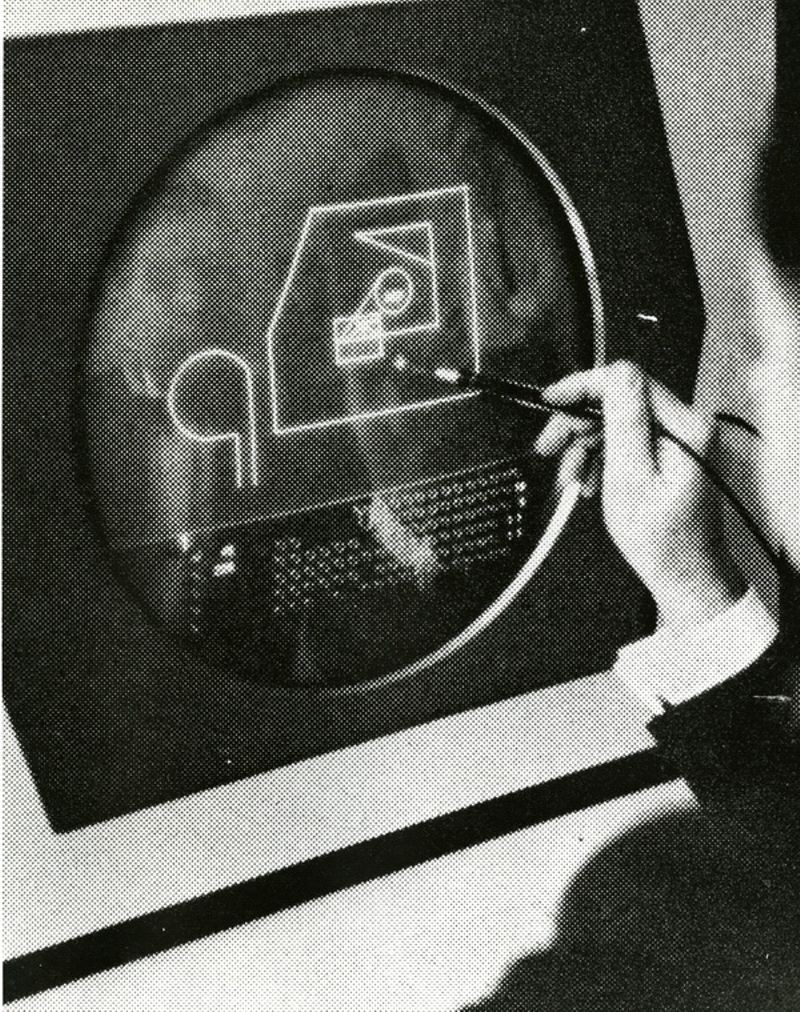
\includegraphics[width=0.4\textwidth]{./graphics/sketchpad-sutherland.jpg} % Change example-image-a with your image filename
  \caption{SketchPad \cite{sutherlandSketchpad}}
\end{wrapfigure}
SketchPad ist ein von Ivan Sutherland entwickeltes Programm, das 1963 am MIT veröffentlicht wurde. 
Es benutzt einen Lightpen als Eingabegerät und war das erste Programm, das die Interaktion mit einem Computer über eine grafische Benutzeroberfläche ermöglichte. 
Es erlaubte den Nutzer/innen, geometrische Formen auf einem Bildschirm zu zeichnen und diese zu manipulieren.
  Dabei existierten diese Formen auf einem virtuellen \qt{Papier}, das der Nutzer bewegen und zoomen konnte. Dieses Konzept von Bewegen und Zoomen virtueller Oberflächen war revolutionär für die damalige Zeit.
  Dies wird deutlich durch den Fakt, dass der Präsentator während der Präsentation von SketchPad \cite{sketchpadDemo} (10:30) keine Worte fand, diesen Vorgang zu beschreiben. Das Konzept von bewegbaren und zoombaren virtuellen Oberflächen ist heute Standard in vielen Anwendungen und wird auch ihm Rahmen dieser Arbeit verwendet.
Ein weiteres Feature war die Möglichkeit, Constraints zwischen den Formen zu definieren, ähnlich wie in modernen CAD-Programmen. 
Wenn man sich die Videodemo von SketchPad anschaut, fallen viele Paradigmen auf, die wir heute als gegeben ansehen.
Auch wenn SketchPad nicht direkt in die Definition einer VPL passt, war es ein Meilenstein der Entwicklung von grafischen HCIs. Was durch die Verleihung des Turing Awards an Ivan Sutherland 1988 bestätigt wurde.
\end{minipage}
\endgroup

\subsubsection{Pygmalion (1970)}
\begingroup
\setlength\intextsep{2pt}
\begin{minipage}{\linewidth}
\begin{wrapfigure}{L}{0.4\textwidth}
  \centering
  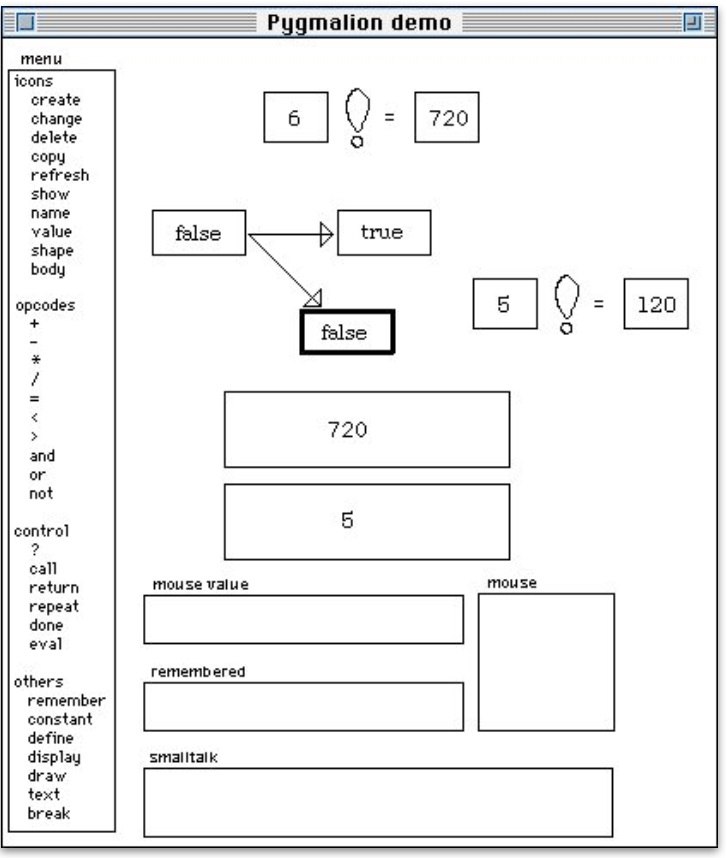
\includegraphics[width=0.4\textwidth]{./graphics/pygmalion.jpg}
  \caption{Fakultät in Pygmalion \cite{smith1975pygmalion}}
  \label{fig:pygmalion_demo}
\end{wrapfigure}

Pygmalion ist eine visuelle Programmiersprache, die um 1970 von David Canfield Smith im Rahmen seiner Doktorarbeit entwickelt wurde. Inspiriert wurde sie vom antiken Bildhauer Pygmalion der seine Skulpturen, dem Mythos nach, zum Leben erwecken konnte.
Die Sprache erlangte nie eine große Verbreitung, war aber ein wichtiger Meilenstein in der Entwicklung von visuellen Programmiersprachen und HCIs.
Pygmalion wurde in Smalltalk implementiert und war eine der ersten visuellen Programmiersprachen. Über eine grafische Oberfläche konnten die Nutzer/innen Blöcke, Icons und Verbindungen erstellen sowie manipulieren, um somit Programme zu definieren.
  Icons waren damals eine Neuerung und wurden von den Entwicklern als \qt{eine Art von visuellen Variablen} bezeichnet. 
  Die Sprache war eine der ersten Beispiele von \qt{Programming By Example} (PBE). Außerdem war sie eine der ersten Sprachen, welche die Verbindung zwischen bestimmten Elementen durch Linien und Pfeile darstellte, was heute ein Standard in vielen VPLs ist.
Die Nutzer/innen konnten Programme schreiben, indem sie die gewünschte Funktionalität in einem Beispiel demonstrieren. 
In Abbildung \ref{fig:pygmalion_demo} wird auf diese Art und Weise die Fakultät einer Zahl berechnet. 

\end{minipage}
\endgroup

\subsubsection{Cube (1996)}

\begingroup
\setlength\intextsep{2pt}

\begin{minipage}{\linewidth}
\begin{wrapfigure}{R}{0.4\textwidth}
  \centering
  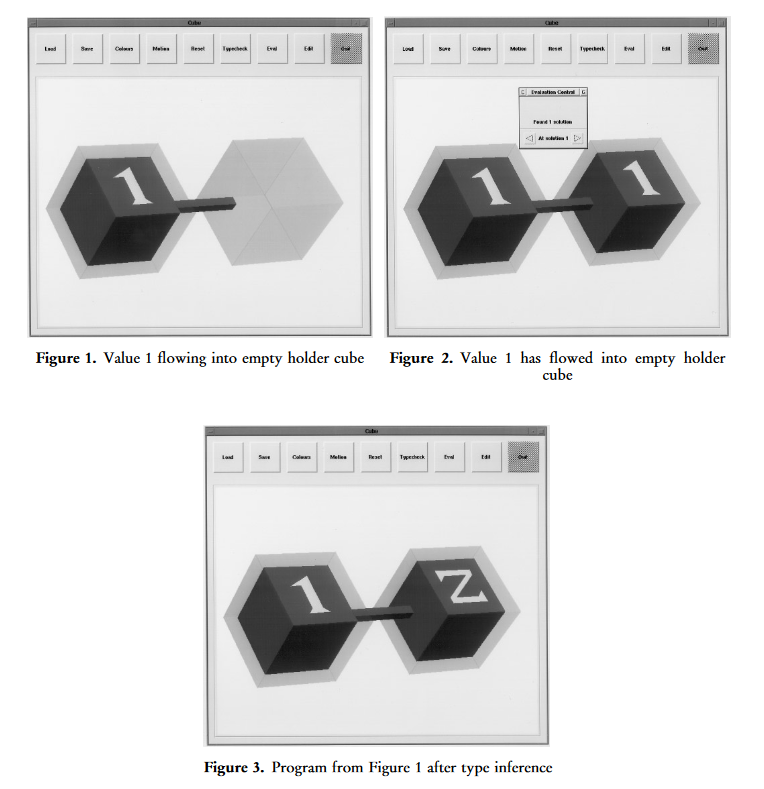
\includegraphics[width=0.4\textwidth]{./graphics/cube_vpl.png} % Change example-image-a with your image filename
  \caption{Datenfluss in Cube \cite{najork1996programming}}
  \label{fig:cube_demo}
\end{wrapfigure}
  \qt{Cube ist eine dreidimensionale, visuelle, statisch typisierte Programmiersprache höherer Ordnung, die für den Einsatz in einer auf virtueller Realität basierenden Programmierumgebung entwickelt wurde.}  \cite{najork1996programming}
In \textit{Cube} werden einzelne Funktionen als, wie der Name schon verrät, Würfel dargestellt. Die Nutzer/innen können diese Cubes miteinander verbinden, um Programme zu erstellen.
  Canfield geht in seiner Arbeit spezifisch auf den Vergleich zu Rohren und Wasserfluss ein. Somit bedient sich \textit{Cube} einer für Menschen relativ intuitiven Darstellung von Wasserfluss durch Rohre, um den Datenfluss innerhalb des Programms darzustellen. Auch dieses Konzept ist relevant für die spezifische Art von visueller Programmiersprache, die in dieser Arbeit entwickelt wird.
  Ein interessantes Detail hierbei ist, dass diese \qt{Rohre} keine Richtung haben und Daten in beide Richtungen fließen können. 
Da \textit{Cube} eine höhere Programmiersprache ist, können die Cubes auch als Argumente an andere Cubes übergeben werden. Dies ermöglicht es, komplexe Programme zu erstellen, die aus vielen einzelnen Cubes bestehen. 
\br
Dieses Konzept ist relevant für meine persönliche Arbeit, siehe \link[parameter_nodes]{parametrisierte Nodes}.

\end{minipage}
\endgroup
\pagebreak

\subsection{Moderne node-basierte visuelle Programmiersprachen}
Die Recherche nach modernen VPLs konzentriert sich spezifisch auf node-basierte VPLs, die entweder durch ihre Popularität oder ihre Spezifizierung relevant für diese Arbeit sind.

\subsubsection{Node-RED}

Node-RED ist eine webbasierte Programmier- und Ausführungsumgebung, die auf Nodes basiert und es den Nutzern ermöglicht, diese Nodes miteinander zu verknüpfen, um \qt{Flows} zu erstellen. 
Es wurde 2013 von IBM entwickelt und ist seit 2016 Teil der OpenJS Foundation (damals JS Foundation).
\cite{nodered}

\begin{figure}[htbp]
  \centering
  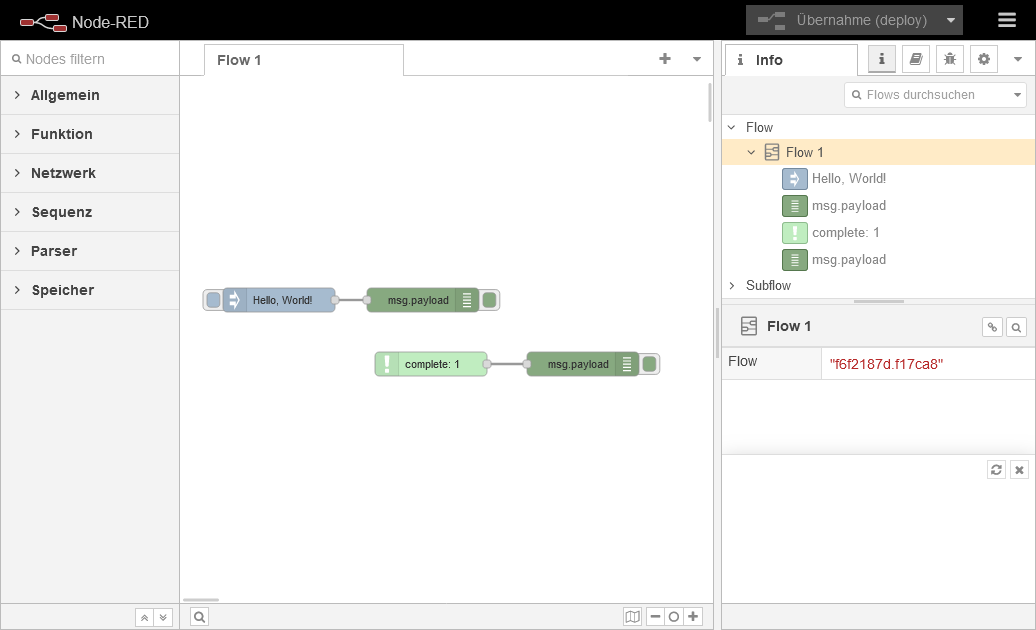
\includegraphics[width=0.7\textwidth]{./graphics/node-red-3_1_8.png}
  \caption{Screenshot Node Red v3.1.8}
  \label{fig:node_red}
\end{figure}

Node-RED findet vor allem Anwendung in den Bereichen IoT und Home Automation, da es eine Vielzahl von Anbindungen an verschiedene Geräte und Dienste bietet. 
Node-RED ist ein Beispiel für sogenannte datenstromorientierte Programmierung, bei der die Daten durch die Nodes fließen und diese verarbeiten. Das heißt, es gibt keine einmalige Ausführung, sondern das System kann kontinuierlich Daten verarbeiten und auf externe Events reagieren. Im Gegensatz zu der in dieser Arbeit entwickelten VPL ist Node-RED nicht auf WebAssembly basiert und ist nicht generalisiert.


\pagebreak
\subsubsection{Blender}
Blender ist eine weitverbreitete Open Source 3D Modellierungs- und Animationssoftware. Die Software bietet node-basierte Interfaces zur Erstellung von Materialien, Texturen und Geometrien. 
\cite{blender}
Für diese Arbeit ist Blender relevant, da die Applikation auch das Erstellen von 3D-Modellen ermöglicht.

\begin{figure}[htbp]
  \centering
  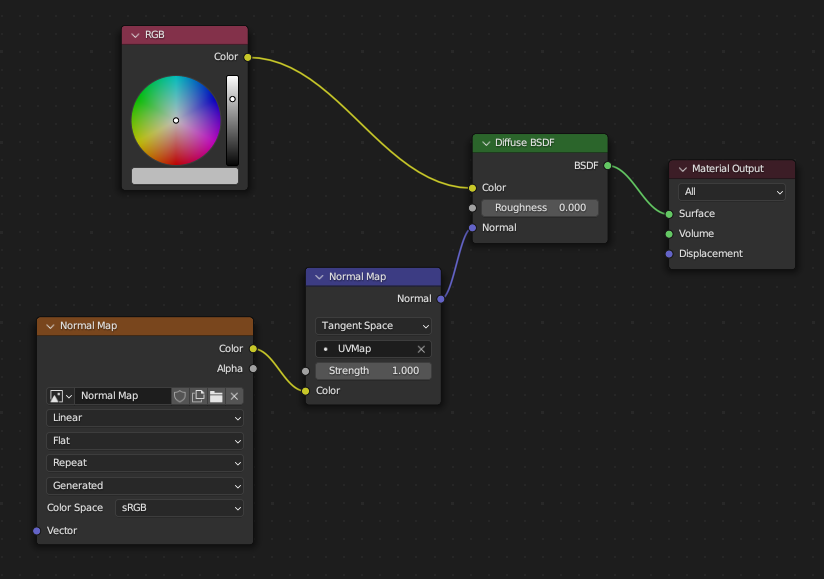
\includegraphics[width=0.6\textwidth]{./graphics/blender-shader.png}
  \caption{Screenshot Blender 3.5 Shader Editor}
  \label{fig:blender-shader}
\end{figure}

Vor allem die User-Experience der Blender Node-Editoren ist ein großer Vorteil. So bietet Blender für die meisten oft benötigten Funktionen Shortcuts an, die es ermöglichen, schnell und effizient zu arbeiten.
Ähnlich wie in Node-RED ist der Datenfluss der westlichen Leserichtung angepasst, von links nach rechts. Dies ermöglicht es, den Datenfluss intuitiv zu verfolgen und zu verstehen.
\br
Im Gegensatz zum Shader Editor (siehe Abbildung \ref{fig:blender-shader}) bietet der Geometry Node Editor die Möglichkeit komplexere Setups zu erstellen. So gibt es zum Beispiel \qt{Repeat Zones}, die es ermöglichen, eine Gruppe von Nodes arbiträr oft zu wiederholen.
\br
Außerdem bietet Blender umfassende Tastaturkürzel an, die es erlauben, sehr schnell und effizient zu arbeiten. In dieser Arbeit soll auch darauf geachtet werden, dass die Nutzer/innen möglichst effizient arbeiten können.

\begin{figure}[htbp]
  \centering
  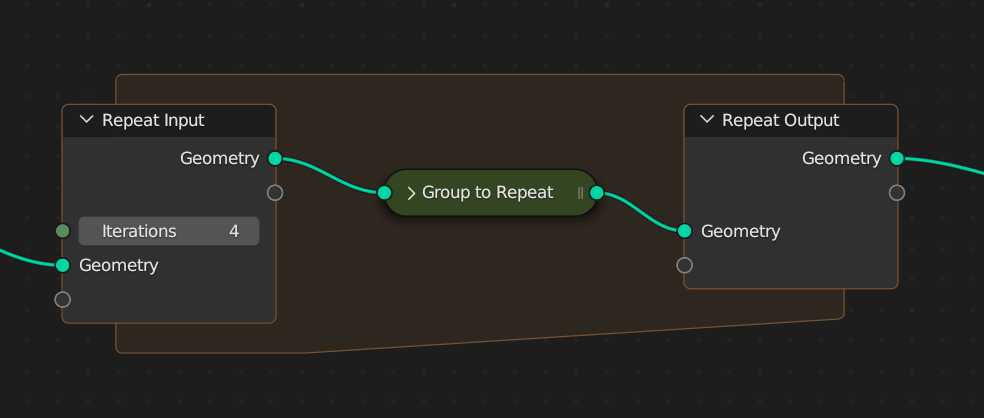
\includegraphics[width=0.6\textwidth]{./graphics/modeling_geometry-nodes_repeat_zone.png}
  \caption{Blender 4.1 Repeat Zone \cite{blenderRepeatZone}}
  \label{fig:blender-repeat}
\end{figure}

\pagebreak

\subsubsection{SpeedTree}

\begin{figure}[htbp]
  \centering
  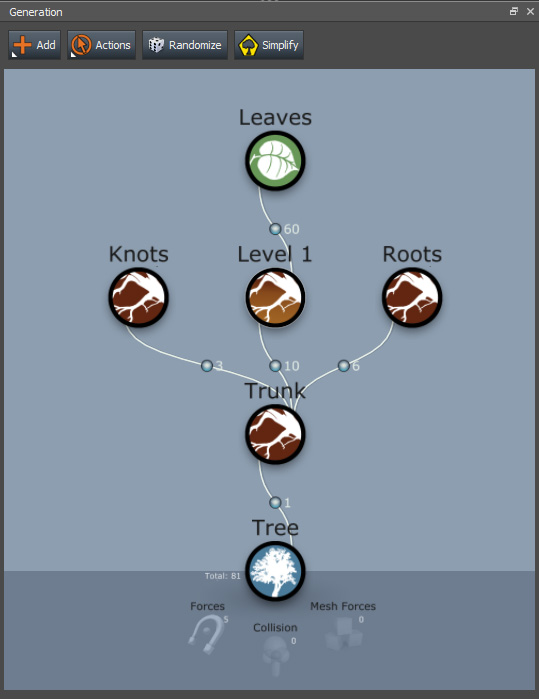
\includegraphics[width=0.6\textwidth]{./graphics/generationeditor_7_speedtree.jpg}
  \caption{SpeedTree Screenshot \cite{speedtreeGettingstartedSpeedTree}}
  \label{fig:blender-repeat}
\end{figure}

SpeedTree ist eine Software zur Erstellung von 3D-Modellen von Pflanzen. Die Nutzer/innen legen über ein node-basiertes Interface die unterschiedlichen Teile eine Pflanze fest und können so sehr detaillierte und realistische Modelle erstellen. SpeedTree wird seit 2000 von Interactive Data Visualization Inc. entwickelt und findet vor allem Anwendung in der Spieleindustrie. \cite{speedtreeGettingstartedSpeedTree}.
\br
Im Gegensatz zu Blender und Node-RED ist SpeedTree ein sehr spezialisiertes Tool. Außerdem ist es nicht Open Source und nicht kostenlos. Auch gibt es keine Möglichkeit, eigene Nodes zu erstellen oder die Software zu erweitern.

\pagebreak

\section{Konzept}
\label{sec:Konzept}

Die in dieser Arbeit entwickelte VPL nutzt einen node-basierten Ansatz. 
\link[node]{Nodes} sind in diesem Kontext einzelne Bausteine, die ähnlich wie eine Funktion in einer textuellen Programmiersprache funktionieren.
Das heißt, sie nehmen Argumente entgegen, verarbeiten diese und geben ein Ergebnis zurück.
\br
Die einzelnen Argumente können entweder direkt über das Interface einer \link[node]{Node} definiert werden oder in dem der/die Nutzer/in das Ergebnis einer anderen \link[node]{Node} mit diesem Argument verknüpft.
Bei der visuellen Gestaltung lehnt sich die VPL an die verschiedenen Node-Editoren in Blender an.
\br
Die einzelnen \link[node]{Nodes} sind hierbei jeweils Instanzen eines WebAssembly-Moduls. 
Dies erlaubt es, das System um neue Node-Definitionen zu erweitern, indem man eine einzelne WebAssembly Dateien lädt.
Woher diese Dateien kommen ist dabei egal, sie können von der Festplatte, einem Server oder aus dem lokalen Speicher geladen werden.
\br
Die Verbindungen mehrerer \link[node]{Nodes} stellen einen \link[node_graph]{Node-Graph} dar. 
Dieser \link[node_graph]{Node-Graph} kann als JSON-Objekt serialisiert und deserialisiert und so gespeichert und geladen werden.
\br
In Abbildung \ref{sec:PURE_GRAPH} ist ein Beispiel für einen \link[node_graph]{Node-Graph} dargestellt. 
Der Datenfluss ist von links nach rechts und die Verbindungen zwischen den Nodes sind gerichtet. In Anlehnung an \link[cube]{Cube} und an die westliche Leserichtung soll so der Datenfluss intuitiv verfolgt werden können.


\begin{figure}[htbp]
    \centering
    \begin{minipage}[b]{0.8\textwidth}
        \centering
        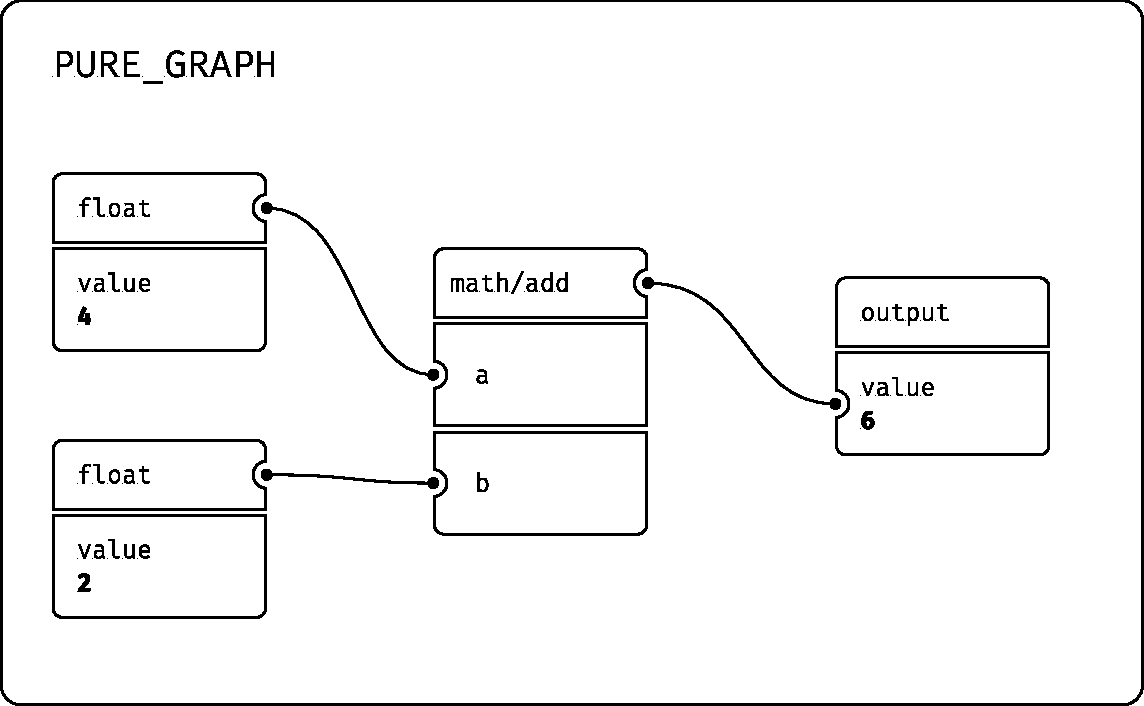
\includegraphics[width=\textwidth]{graphics/PURE_GRAPH.pdf}
        \caption{Darstellung eines \link[node_graph]{Node-Graph}}
        \label{sec:PURE_GRAPH}
    \end{minipage}
\end{figure}

\pagebreak


\subsection{Architektur}
\label{sec:Architektur}
Aus den drei \link{Anforderungen}, \textbf{performant}, \textbf{erweiterbar} und \textbf{einfach zu benutzen} sowie dem \link{Konzept} ergibt sich folgende dreiteilige Architektur:
\br
Das \textbf{\link[node_interface]{Node-Interface}} ist für das visuelle Interface zuständig, hier interagieren Nutzer/innen mit dem \link[node_graph]{Node-Graph}.
\br
Der \textbf{\link[runtime_executor]{Runtime-Executor}} ist für die Ausführung der Nodes zuständig. Er nimmt einen serialisierten \link[node_graph]{Node-Graph} entgegen und gibt das Ergebnis zurück.
\br
Die \textbf{\link[node_registry]{Node-Registry}} ist für das Verwalten der \link[node_definition]{Node-Definitionen} zuständig. Die beiden anderen Komponenten laden aus ihr die einzelnen WebAssembly-Binärdateien der Nodes.
\br
Das System wurde in diese drei Komponenten unterteilt, da sich so der Datentransfer zwischen den einzelnen Komponenten minimieren lässt, die Komponenten lose gekoppelt sind und dadurch einfacher ersetzt oder erweitert werden können.
In Abbildung \ref{fig:overview_sequence} ist in einem Sequenzdiagramm dargestellt, wie die drei Komponenten zusammenarbeiten.

\begin{figure}[hbtp]
    \centering
    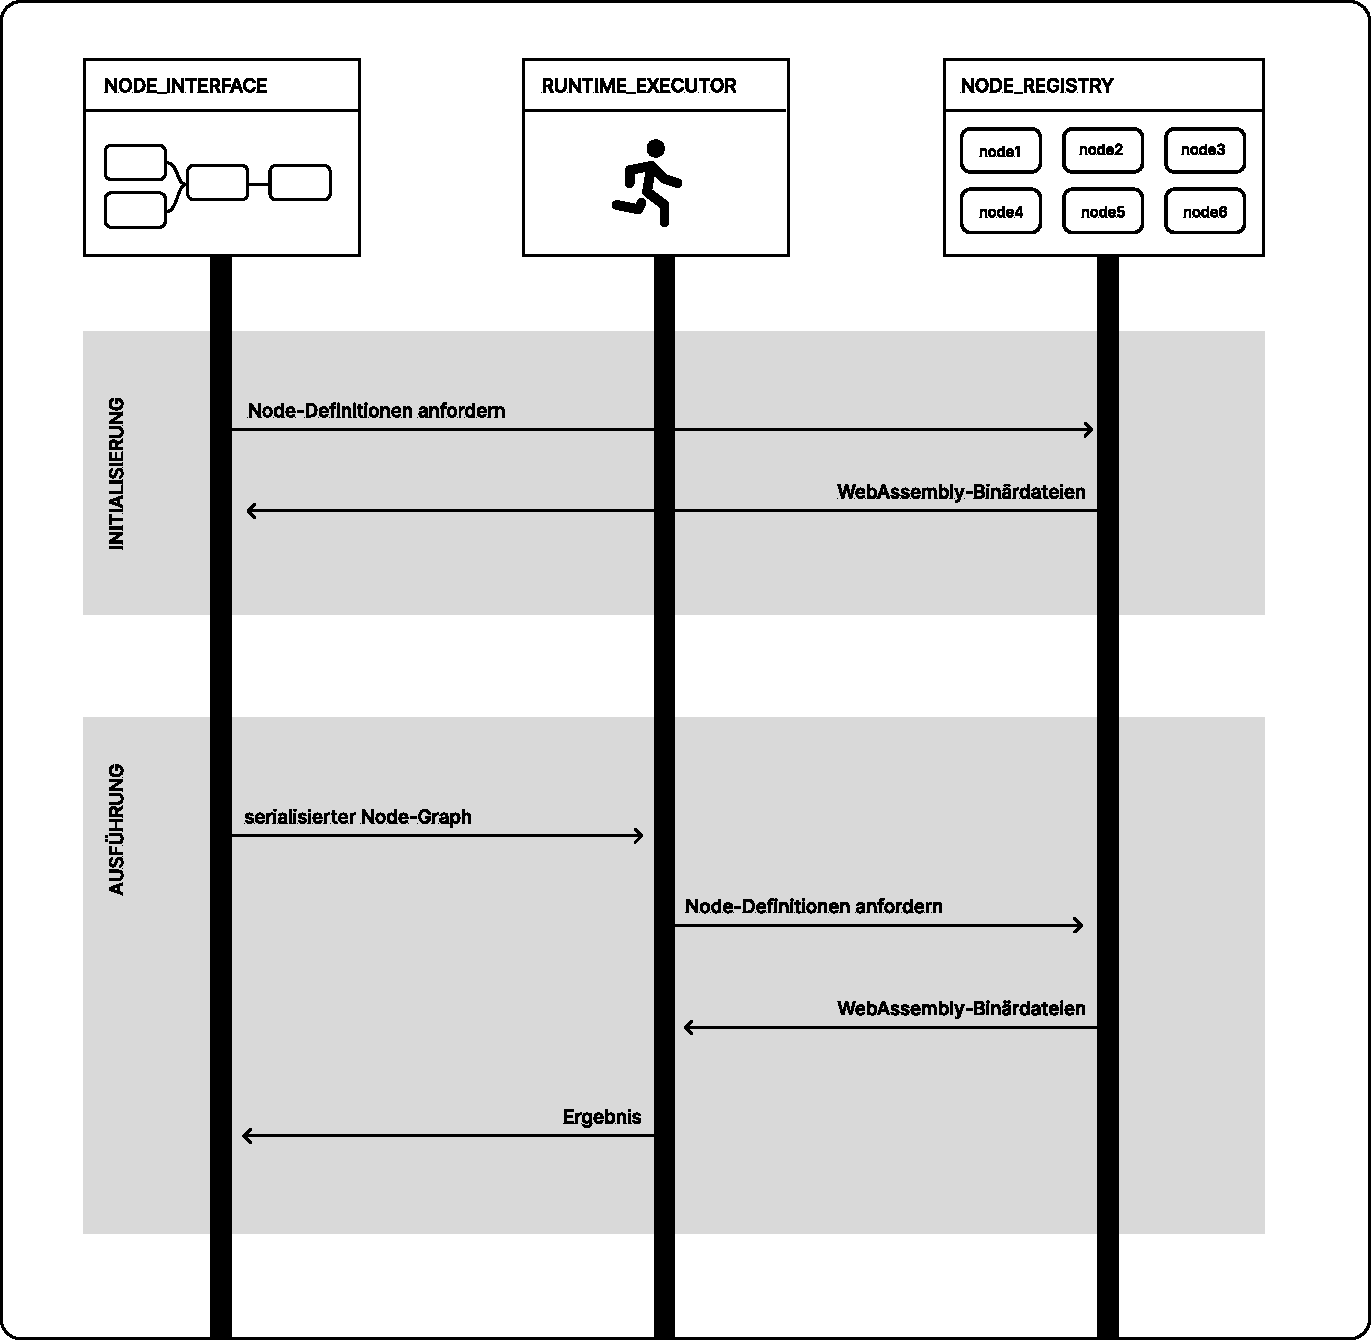
\includegraphics[width=0.85\textwidth]{graphics/OVERVIEW_SEQUENCE.pdf}
    \caption{Sequenzdiagramm der Architektur}
    \label{fig:overview_sequence}
\end{figure}

\pagebreak

\subsubsection{Datentypen}

Die Datentypen wurden möglichst minimal gehalten. Dies dient zum einen dem Ziel, das gesamte System so einfach und verständlich wie möglich zu halten, und zum
anderen beschleunigt es die Serialisierung, Deserialisierung und den Transfer der Daten.
\br
Die drei Hauptdatentypen sind  \link[data_node_type]{Node-Definition}, \hyperref[fig:data_node]{Node},  und \hyperref[fig:data_node_graph]{Node-Graph}. 

\subsubsection*{Node-Definition}

\begin{figure}[htbp]
  \begin{code}
    \begin{minted}{typescript}
type NodeDefinition = {
  id: string;
  inputs?: Record<string, NodeInput>
  outputs?: string[];
  execute?: (args: Int32Array) => Int32Array;
}

// Beispiel einer Math Node
const mathNodeType: NodeDefinition = {
  id: "max/plantarium/math",
  inputs: { 
    op_type: { type:"select", options: ["add","subtract","multiply","divide"] }, 
    a: { type: "float" }, 
    b: { type: "float" } 
  },
  outputs: ["float"],
  execute: (inputs) => {
    // Implementierung der Math Node
  }
}
    \end{minted}
  \end{code}

  \caption{Datenstruktur der \link[node_definition]{Node-Definition} (TypeScript)}
  \label{sec:data_node_type}

\end{figure}

Die Node-Definition besteht aus einer \topic{id}, \topic{inputs}, \topic{outputs} und einer \topic{execute}-Funktion. Die \topic{inputs} einer \link[node]{Node} können unterschiedliche \topic{type} Werte haben, beispielsweise:

\begin{itemize}
  \setlength\itemsep{0.0em}
  \item float
  \item integer
  \item boolean
  \item select
  \item vec3
\end{itemize}

Über diese \topic{inputs} wird festgelegt, welche Argumente eine \link[node]{Node} entgegennimmt.
Im \link[node_interface]{Node-Interface} werden diese als Eingabefelder dargestellt. Außerdem legen diese Inputs fest,  welche \link[node]{Nodes} mit dieser \link[node]{Node} verbunden werden können. 
\br
Ein weiteres Attribut eines \topic{inputs} ist \topic{setting}. So können die Nutzer Argumente festlegen, die global für den ganzen \link[node_graph]{Node-Graph} gelten und nicht direkt von einer \link[node]{Node} abhängen. Ein Beispiel aus der Entwicklung wäre hier die \topic{resolution}. Diese legt fest, wie viele Vertices eine \link[node]{Node} für ein 3D-Modell generieren soll. Das \link[node_interface]{Node-Interface} konstruiert aus allen \topic{settings} ein globales Einstellungsmenü.
\br
Außerdem gibt es bestimmte Input-Typen mit besonderer Funktion. So kann eine \link[node]{Node} zum Beispiel einen Input mit \topic{\{"type":\\"\\seed"\}} festlegen. Diesem wird bei der Ausführung durch den \link[runtime_executor]{Runtime-Executor} ein zufälliger Wert zugewiesen.
\br
Einige andere Attribute wurden ausgeklammert, um die Lesbarkeit zu erhöhen. So kann ein \topic{input} noch ein \topic{label}, ein \topic{default} und eine \topic{description} haben.

\subsubsection*{Node}

\begin{figure}[htbp]
  \begin{code}
    \begin{minted}{typescript}
type Node = {
  id: number;                       // Primäre ID der Node
  type: string;                     // Type der Node, bsp: max/plantarium/math
  props?: Record<string, any>,      // Daten der Node
  position: [x: number, y: number]  // Visuelle Position
}

const exampleNode: Node = {
  id: 5,
  type: "max/plantarium/math",
  props: { op_type: 0, a: 400, b: 20},
  position: [60, 90]
}

    \end{minted}
  \end{code}

  \caption{Datenstruktur einer \link[node]{Node} (TypeScript)}
  \label{fig:data_node}

\end{figure}

Eine \link[node]{Node} ist eine Instanz einer \link[node_definition]{Node-Definition}. Die Datenstruktur besteht aus einer \topic{id}, einem \topic{type}, optionalen \topic{props} und einer \topic{position}. 
Dieser Datentype findet vor allem im \link[node_interface]{Node-Interface} Anwendung – während der Laufzeit und der Serialisierung und Deserialisierung.
\br
Die \topic{id} ist inkrementell und dient zur eindeutigen Identifikation der Node. Der \topic{type} verbindet eine \link[node]{Node} mit einer \link[node_definition]{Node-Definition}.
Die \topic{props} sind die Argumente, die an die \topic{execute} Funktion der \link[node_definition]{Node-Definition} übergeben werden.

\subsubsection*{Node-Graph}

\begin{figure}[htbp]
  \begin{code}
    \begin{minted}{typescript}
type NodeGraph = {
  id: number;                                 // Primäre ID des Graphen
  nodes: Node[];                              // Liste aller Nodes
  edges: [number, number, string][];  // Liste aller Verbindungen
}
    \end{minted}
  \end{code}

  \caption{Datenstruktur eines \link[node_graph]{Node-Graph} (TypeScript)}
  \label{fig:data_node_graph}

\end{figure}

Der \link[node_graph]{Node-Graph} besteht aus einer \topic{id}, einer Liste aller \link[node]{Nodes} und einer Liste aller Verbindungen. 
Die Verbindungen sind jeweils ein Tupel, aus der \topic{id} der \link[node]{Node} von der die Verbindung ausgeht, der \topic{id} der \link[node]{Node} zu der die Verbindung geht, und der \topic{id} des \topic{inputs} der empfangenden Node.

\pagebreak

\subsubsection{Node-Interface}
\label{sec:node_interface}

Das Node-Interface ist die Benutzeroberfläche des Systems. Hier können die Nutzer/innen \link[node]{Nodes} erstellen, verbinden und löschen. 
Wichtig ist, dass das Interface so einfach und intuitiv wie möglich ist, um die Nutzer/innen nicht zu überfordern. Gleichzeitig soll es aber auch genug Funktionen bieten, um komplexe Programme zu erstellen. Auch soll es viele Tastaturkürzel und andere Funktionen geben, um die Nutzer/innen möglichst effizient arbeiten zu lassen.

\subsubsection{Node-Registry}
\label{sec:node_registry}

Die \link[node_registry]{Node-Registry} ist für das Verwalten der \link[node_definition]{Node-Definitionen} zuständig. Konzeptuell funktioniert sie ähnlich wie die Package-Manager der gängigen Programmiersprachen, z.B. \href{https://www.npmjs.com/}{npm} oder \href{https://crates.io/}{crates.io}.
\br
Damit diese \link[node_registry]{Node-Registry} erweiterbar ist, wurde ein eigenes ID-Schema für die \link[node_definition]{Node-Definitionen} entworfen. Dies besteht aus einer \topic{user-id}, einem \topic{namespace} und der \topic{node-id}. 
Ein Beispiel aus der Entwicklung wäre \topic{max/plantarium/branch}.
\br
Die \topic{user-id} ist die ID des/der Entwicklers/Entwicklerin und dient dazu, die Nodes zu gruppieren. Der Namespace gruppiert Nodes, die zusammen funktionieren. So kann das System der \link[parameter_nodes]{parametrisierten Nodes} nur für Nodes in dem \topic{plantarium} Namespace implementiert werden und andere Namespaces können andere Implementierungen haben.
\br
Die \topic{node-id} muss individuell innerhalb eines \topic{namespaces} sein. 

\subsubsection*{Non-Goals}
Obwohl im Design darauf geachtet wurde, die \link[node_registry]{Node-Registry} so erweiterbar wie möglich zu machen, wurde darauf verzichtet Funktionen, die eine \qt{echte} Registry benötigt, zu implementieren. So gibt es keine Ansätze zur Versionierung, auch auf Authentifizierung und Autorisierung wurde verzichtet.

\pagebreak

\subsubsection{Runtime-Executor}
\label{sec:runtime_executor}

Der \link[runtime_executor]{Runtime-Executor} ist für die Ausführung eines \link[node_graph]{Node-Graphen} zuständig.

\begin{figure}[htbp]
  \begin{code}
    \begin{minted}{typescript}
export interface RuntimeExecutor {
  /**
  * Execute the given graph
  * @param graph - The graph to execute
  * @returns The result of the execution
  */
  execute: (graph: Graph, settings: Record<string, unknown>) => Promise<Int32Array>;
}
    \end{minted}
  \end{code}
  \caption{Interface des \link[runtime_executor]{Runtime-Executor} (TypeScript)}
  \label{fig:runtime_executor}
\end{figure}

Aus Abbildung \ref{fig:runtime_executor} soll ersichtlich werden, das diese Klasse ein denkbar simples Interface hat. 

\subsubsection{Parametrisierte Nodes}
\label{sec:parameter_nodes}
In vorherigen Abschnitten wurde der Vergleich zwischen \link[node]{Nodes} und Funktionen gezogen. Dies hat den Vorteil, dass es das Konzept etwas leichter verständlich macht.
Es gibt jedoch Situationen, in denen es sinnvoll ist, von dem Konzept einer Node als reiner Funktion abzuweichen, damit die VPL flexibler und intuitiver ist. Die folgenden Abschnitte werden diese Situationen erläutern und eine Lösung vorstellen.

\subsubsection*{Random-Problem}
In Abbildung \ref{fig:random_problem} ist ein beispielhafter Aufbau eines \link[node_graph]{Node-Graphen} dargestellt. Wären die \topic{random} Nodes als reine Funktion implementiert, würde sie nur einmal ausgeführt und die beiden \topic{math/add} Nodes würden das gleiche Ergebnis produzieren. Dies wäre für die meisten Nutzenden ein überraschendes Ergebnis.
\br
Eine mögliche Lösung wäre, die \topic{random} Node für jede ihrer ausgehenden Verbindungen separat auszuführen. 
Dies könnte jedoch zur unnötigen Mehrfachausführung von Nodes führen, die dies nicht erfordern.
Außerdem würde das Caching von Node-Ergebnissen erschwert, da nicht nur die Node-Parameter, sondern auch die Anzahl der ausgehenden Verbindungen das Ergebnis beeinflussen würden.
\br
Ein weiterer Nachteil ist, dass für dieses Konzept die Ausführung der Nodes nicht mehr nur in eine Richtung verläuft. Das könnte zu konzeptioneller Verwirrung und ungewollter Komplexität führen.
\br
\begin{figure}[htbp]
  \centering
  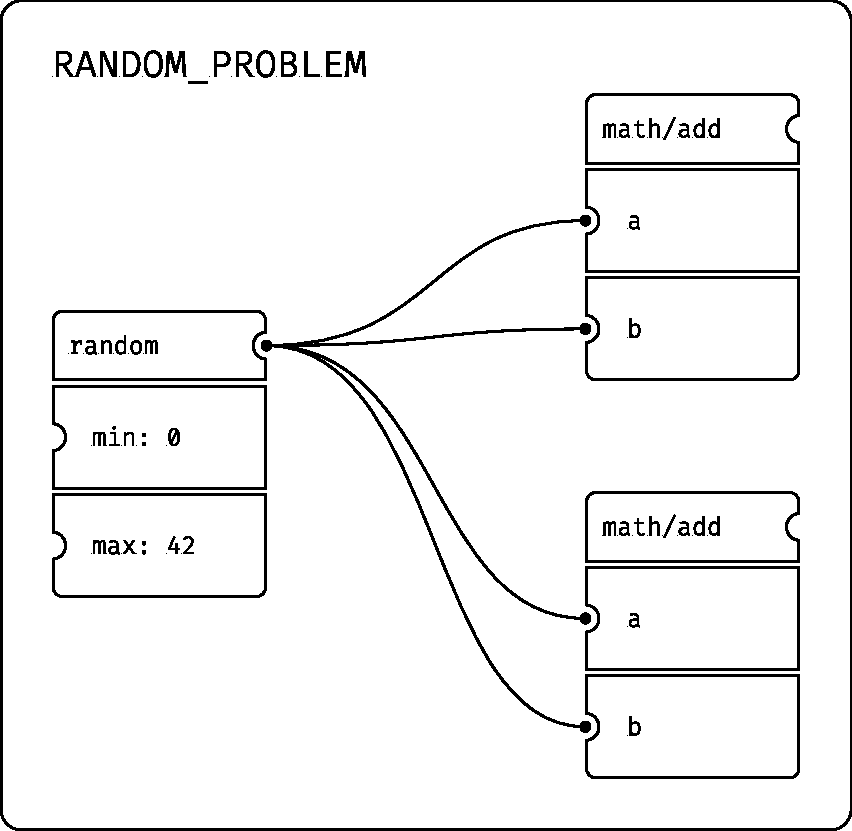
\includegraphics[width=0.5\textwidth]{graphics/RANDOM_PROBLEM.pdf}
  \caption{Illustration eines Problems mit der \topic{random} Node}
  \label{fig:random_problem}
\end{figure}

\pagebreak

\subsubsection*{Noise-Problem}

Ein weiteres Problem soll durch Abbildung \ref{fig:noise_problem} verdeutlicht werden. 
Die hypothetische \topic{cylinder} Node generiert 3D-Modelle von Zylindern. Sie hat einen Input für den Radius, die Höhe und die Anzahl der generierten Zylinder. 
\br
Wenn die vorherigen Nodes als pure Funktionen modelliert wären, würde diese Node Ergebnis A produzieren, da die \topic{noise} Node nur einmal ausgeführt wird. Die meisten Nutzenden würden jedoch eher Ergebnis B erwarten.

\begin{figure}[htbp]
  \centering
  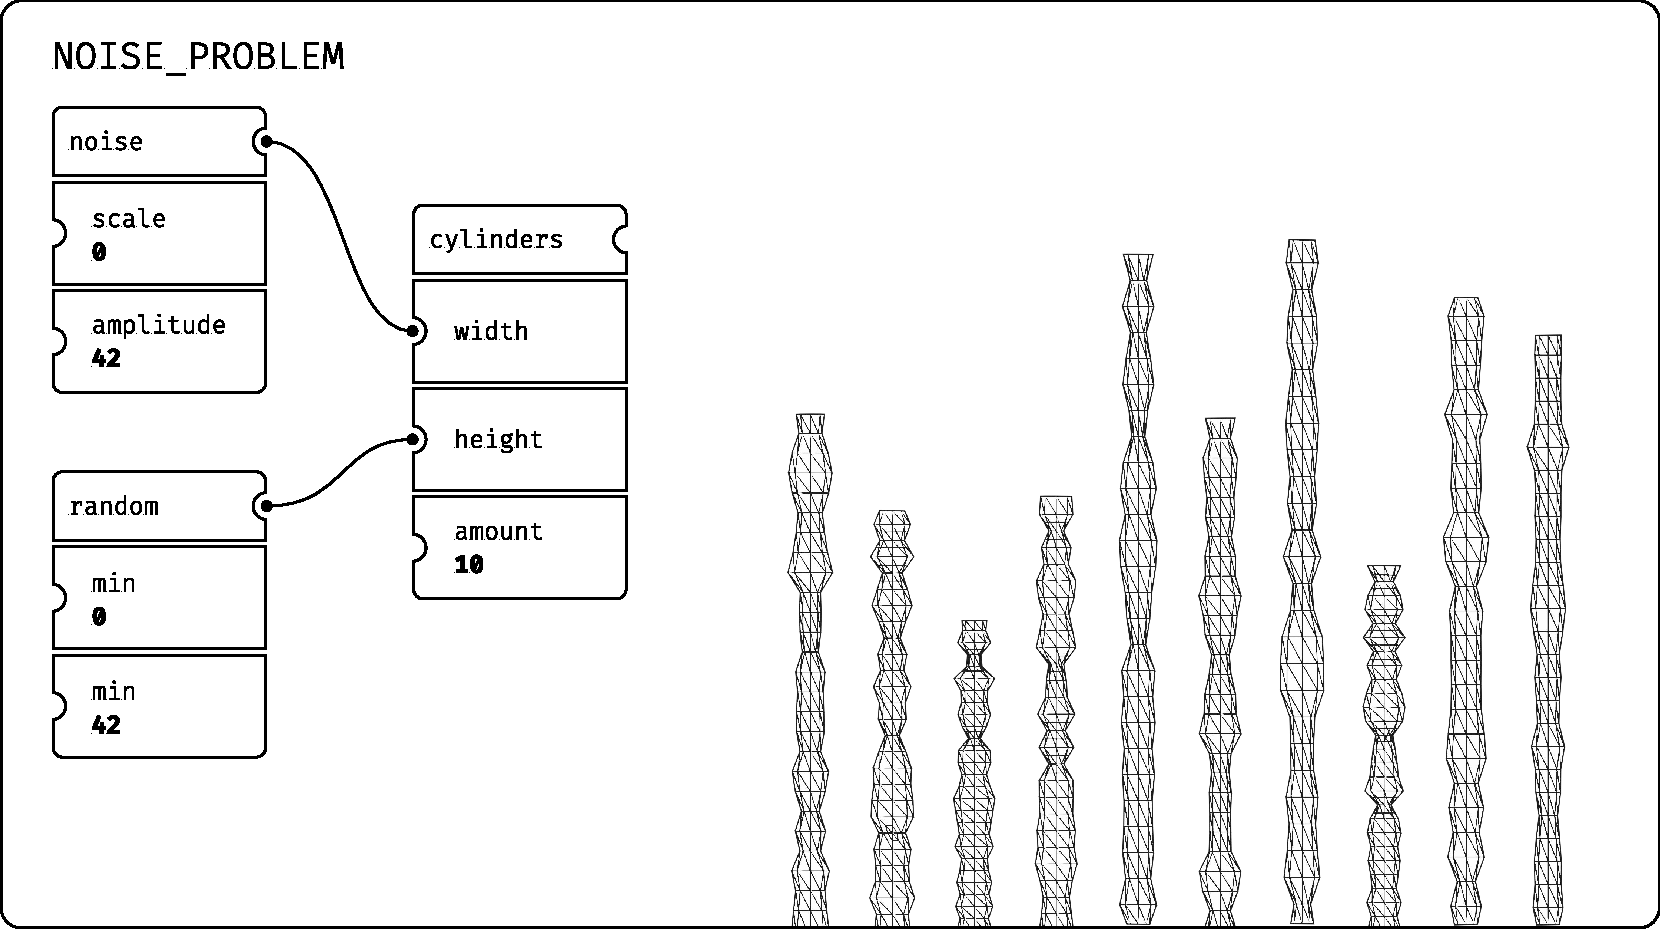
\includegraphics[width=0.8\textwidth]{./graphics/NOISE_PROBLEM.pdf}
  \caption{Problemdarstellung}
  \label{fig:noise_problem}
\end{figure}

\subsubsection*{Lösung}

Eine Lösung für dieses Problem ist die Einführung von parametrisierten Nodes. Das heißt, bestimmte Nodes geben kein Ergebnis zurück, sondern eine parametrisierte Version ihrer selbst, die dann von anderen Nodes evaluiert werden kann.
\br
Dies hat den entscheidenden Vorteil, dass andere Nodes frei entscheiden können, wo und wie oft sie ihre Argumente evaluieren.
Außerdem kann dies implementiert, ohne die Runtime zu beeinflussen, da die Ausführung der Nodes weiterhin in einer Richtung verläuft.
\br
Die \topic{cylinder} Node im vorherigen Beispiel könnte zum Beispiel bei der Evaluierung der \topic{random} Node ein \topic{seed} übergeben.
\br
Eine Herausforderung in der Implementierung dieser Lösung besteht darin, dass jedes Argument nun entweder ein direkter Wert, der von den Nutzern über das \link[node_interface]{Node-Interface} festgelegt wird, oder ein Teil des gesamten \link[node_graph]{Node-Graphen} sein kann.
\br
Die erste Implementierung bestand darin, dass die Nodes ein serialisiertes JSON-Objekt zurückgeben. Dies hatte den Vorteil, dass einzelne Argumente zu Debugging-Zwecken menschenlesbar und die Serialisierung relativ einfach war. Die Performance war jedoch nicht optimal, da die Serialisierung und Deserialisierung relativ aufwendig ist. Des Weiteren hatte jede Node jetzt eine Abhängigkeit zu \href{ https://serde.rs/ }{Serde} (Der Standardbibliothek für Serialisierung in Rust), was die Dateigröße der WebAssembly-Module deutlich vergrößerte.
\br
Die aktuelle Version benutzt eine eigene Binär-Serialisierung. Diese ist schneller und die Dateigröße der WebAssembly-Module ist kleiner. Der Nachteil ist, dass die Serialisierung nicht mehr menschenlesbar und die Implementierung komplexer ist. 
\br
Die Grundidee ist es, Nodes als ein Array aus 32-Bit-Integer darzustellen. Die erste Stelle des Arrays enkodiert den Typ der Node, die darauffolgenden Stellen sind die Argumente. Die einzelnen Argumente sind entweder eine Zahl oder die enkodierte Version einer anderen Node.
Gleitzahlen sind 32-Bit nach dem IEEE-754 Standard und können dank der gleichen Größe ohne weitere Anpassungen im Array gespeichert werden. 
\br
Da WebAssembly, sowie auch Rust keine verschachtelten Arrays unterstützen, muss dieser Array in einen linearen Array umgewandelt werden. 
Bei meiner Recherche nach existierenden Algorithmen zu diesem Problem, bin ich auf den \qt{Recursive-Length Prefix Serialization} (RLP)-Algorithmus von Ethereum gestoßen. Dieser Algorithmus war ein guter Ansatz, ist jedoch nicht für die Anforderungen dieser Anwendung optimiert, da er nur Arrays unterstützt, die entweder Nummern oder Arrays enthalten und keine gemischte Version. Außerdem ist er für das Enkodieren von Strings optimiert.
\cite{wood2024ethereum}
\br
Das aktuelle Binärformat besteht darin, jede Klammer in einem verschachtelten Array durch zwei 32-Bit-Integer zu enkodieren. 
Die erste Stelle gibt an, ob es sich um eine öffnende oder schließende Klammer handelt, die zweite Stelle gibt den Abstand zur nächsten Klammer an.

\begin{figure}[htbp]
  \centering
  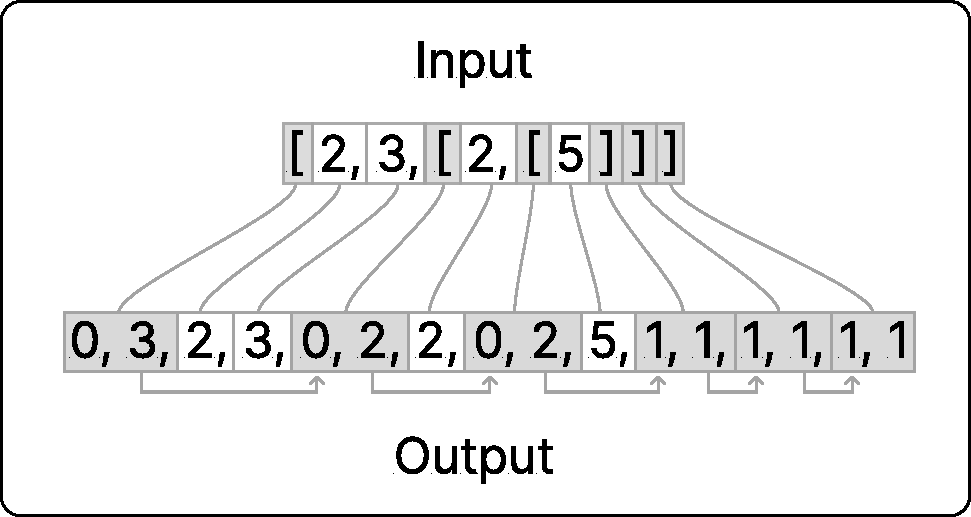
\includegraphics[width=0.8\textwidth]{./graphics/ENCODING_SCHEME.pdf}
  \caption{Visualisierung der Binär-Serialisierung}
  \label{fig:encoding_scheme}
\end{figure}

Eine Limitierung dieser Implementierung ist, dass signierte 32-Bit-Integer nur Zahlen bis maximal $2^{31}-1$ darstellen können. Dies beschränkt die Länge eines Arrays auf $2,147,483,647$ Elemente. Für diese Anwendung ist das jedoch mehr als ausreichend.

\subsubsection*{O-Notation}
Die O-Notation der \link[code_nested_encoding]{Beispiel-Implementierung} ist $O(n)$, wobei $n$ die Anzahl der Elemente in der Serialisierung ist. Tatsächlich können wir aber während der Laufzeit oft einen einfacheren Algorithmus benutzen, da die meisten parametrisierten Nodes nicht tief in die Verschachtelung gehen, sondern nur die obersten Elemente extrahieren und nachher wieder zusammenfügen. 
\br
Beispielsweise nimmt eine \topic{math} Node, ihre Operation (addieren, subtrahieren...) und zwei Zahlen entgegen und fügt diesen Argumenten nur einen Integer zur Identifizierung des Node-Typen hinzu. Dafür können wir Algorithmen benutzen, die nur die obersten Elemente \link[code_nested_splitting]{extrahieren} und wieder \link[code_nested_joining]{zusammenfügen}.  Diese Algorithmen haben eine O-Notation von $O(1)$.

\pagebreak

\subsection{Design}

Die Anwendung wurde so designt, dass sie möglichst einfach und intuitiv zu bedienen ist. Dafür wurde ein simples, zweispaltiges Layout gewählt. Auf der rechten Seite befindet sich das \link[node_interface]{Node-Interface} und auf der linken Seite die 3D-Visualisierung der entstandenen Pflanze. Zudem gibt es auf der rechten Seite eine Symbolleiste, die den Zugriff auf verschiedene Untermenüs erlaubt. Diese sind standardmäßig ausgeblendet, um die Übersicht zu erhöhen.

\begin{figure}[hbtp]
  \centering
  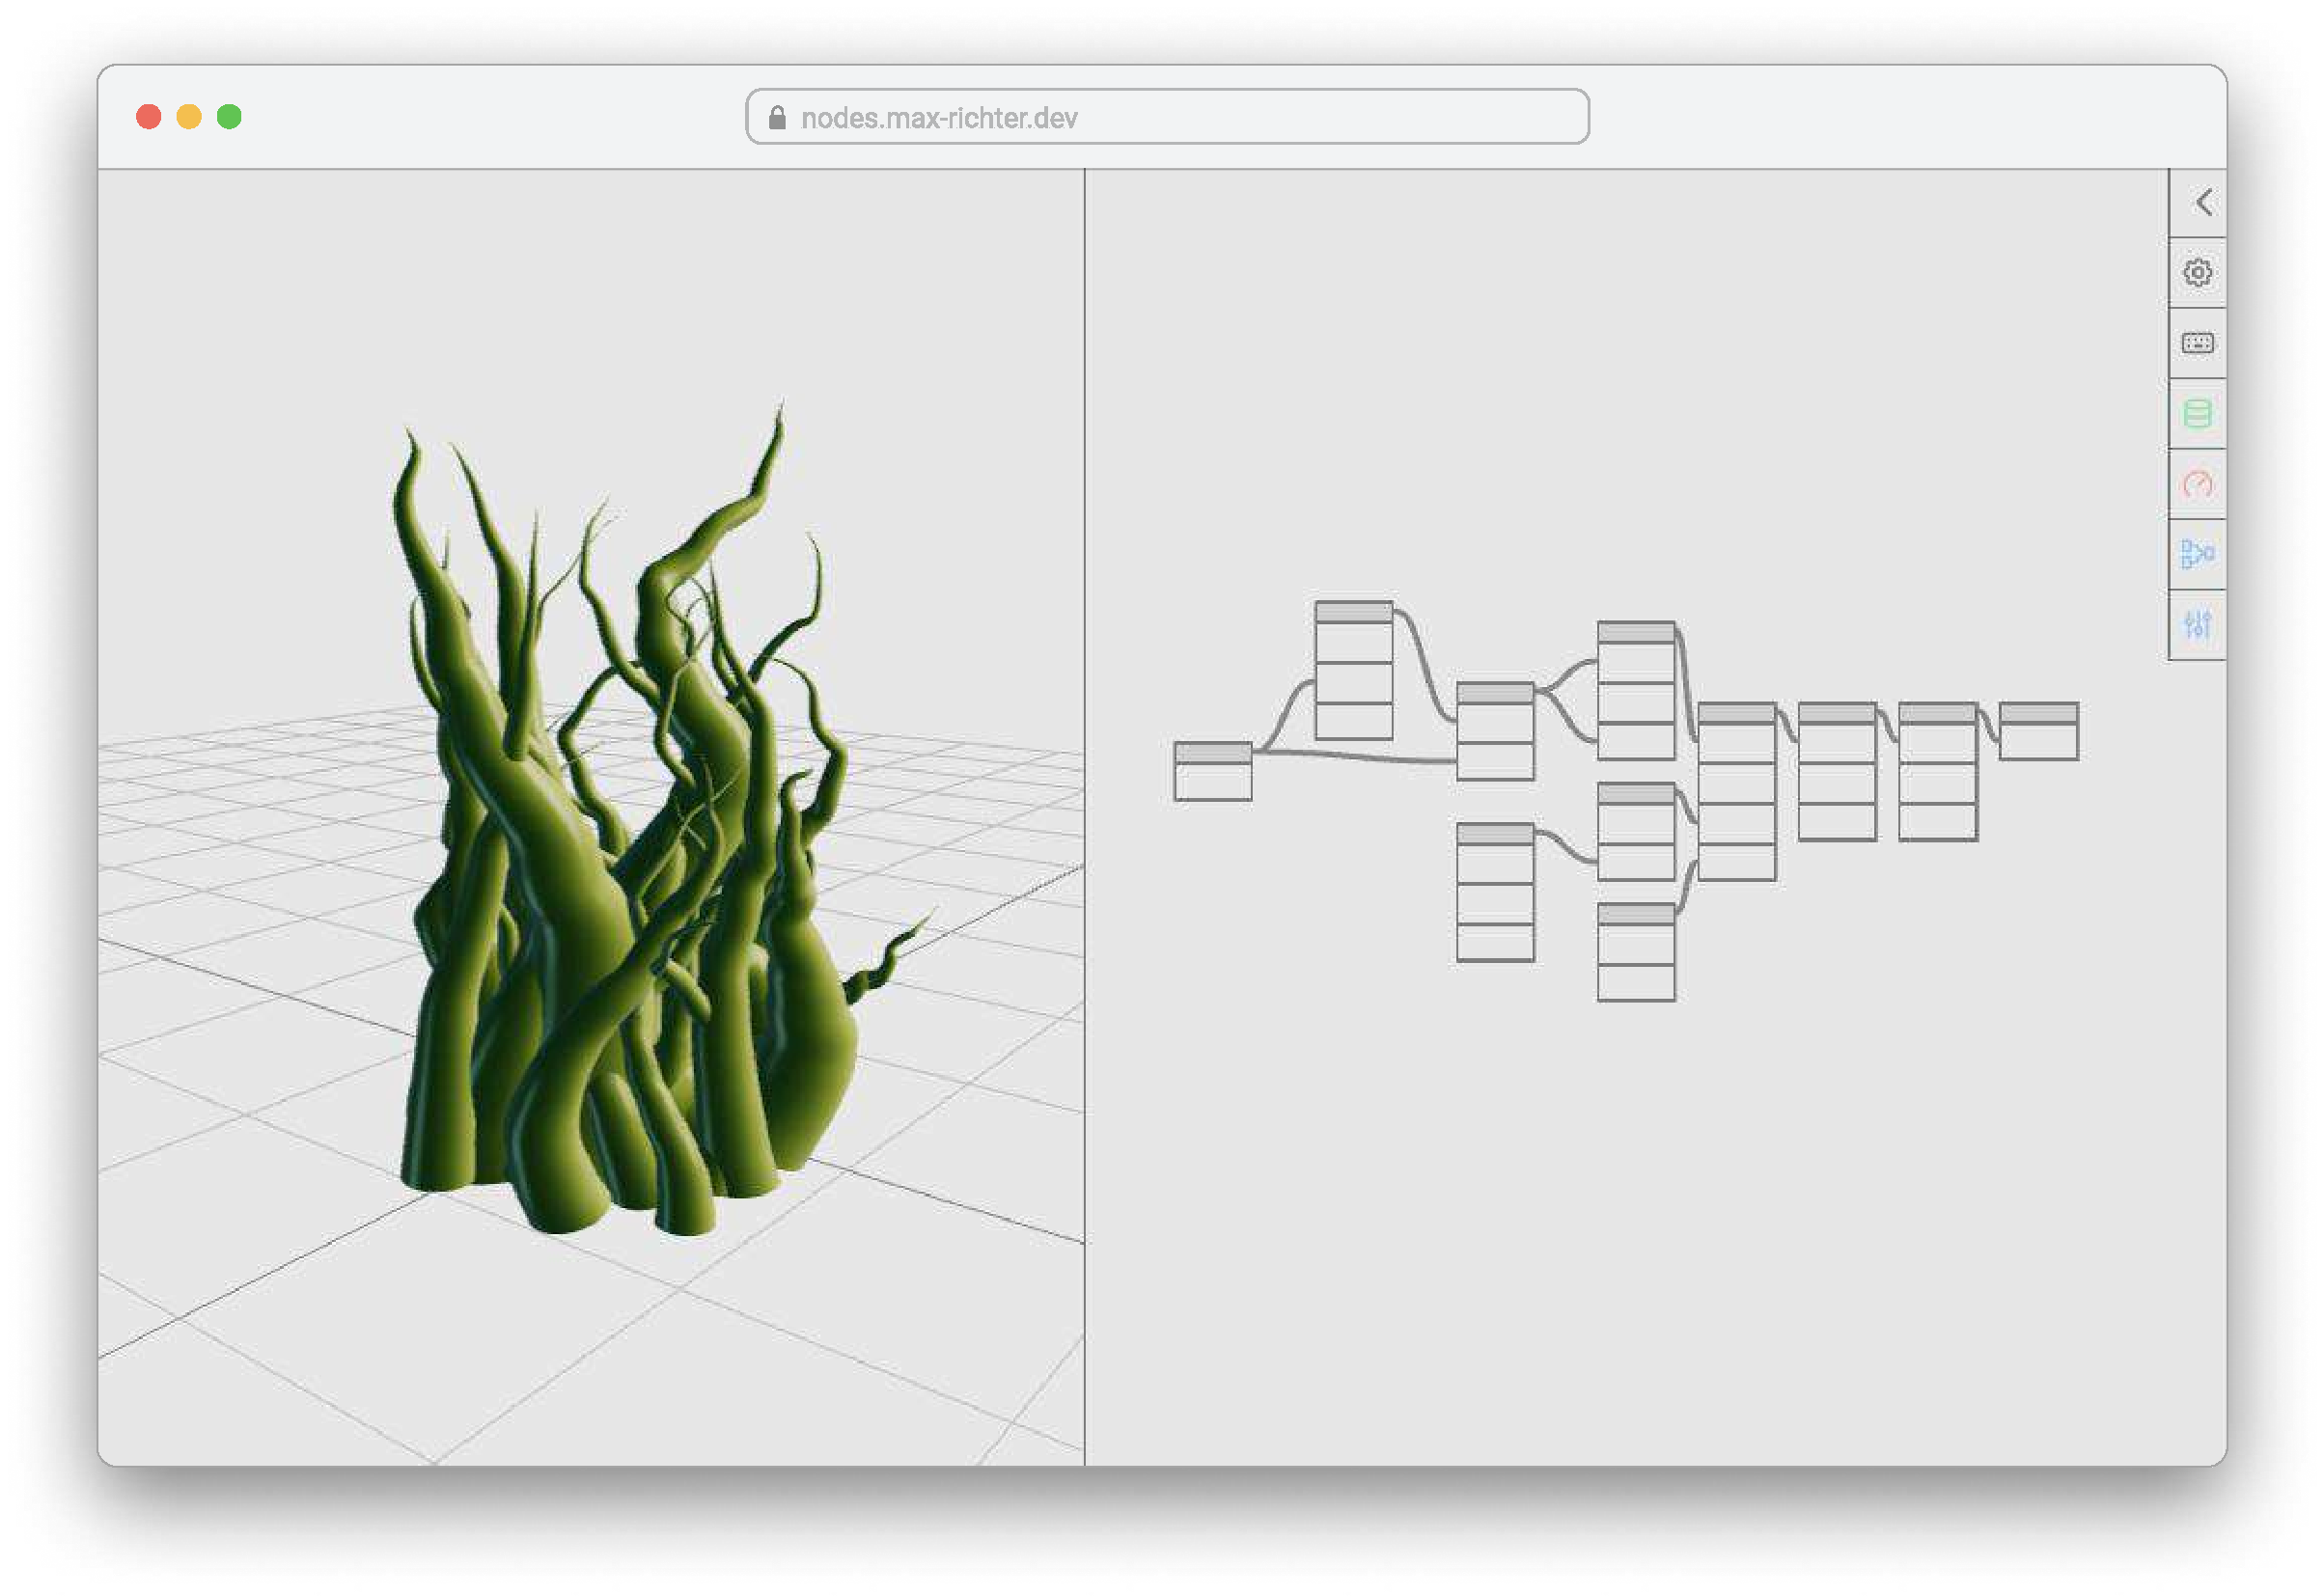
\includegraphics[width=1\textwidth]{graphics/layout_light.pdf}
  \caption{Screenshot der Anwendung im Light-Mode}
  \label{fig:screenshot_nodarium}
\end{figure}

\subsubsection{Farbgebung}

Da es sich bei der Anwendung um ein Tool für die Entwicklung von 3D-Modellen handelt, wurde eine  möglichst unaufdringliche und minimalistische Farbgebung entworfen.
Zur Entwicklung der Farbpalette wurde ein neutrales dunkles Grau gewählt, aus dem zwei dunklere und drei hellere Farben abgeleitet wurden. Aus diesen 6 Farbtönen wurden dann die einzelnen Farbschemata für die Anwendung abgeleitet. Außerdem wurde ein High-Contrast-Mode implementiert, der die Farben so anpasst, dass sie auch für Nutzer/innen mit Sehschwäche gut erkennbar sind.

\subsubsection{Node-Design}


\begingroup
\setlength\intextsep{4pt}
\begin{minipage}{\linewidth}
\begin{wrapfigure}{L}{0.48\textwidth}
    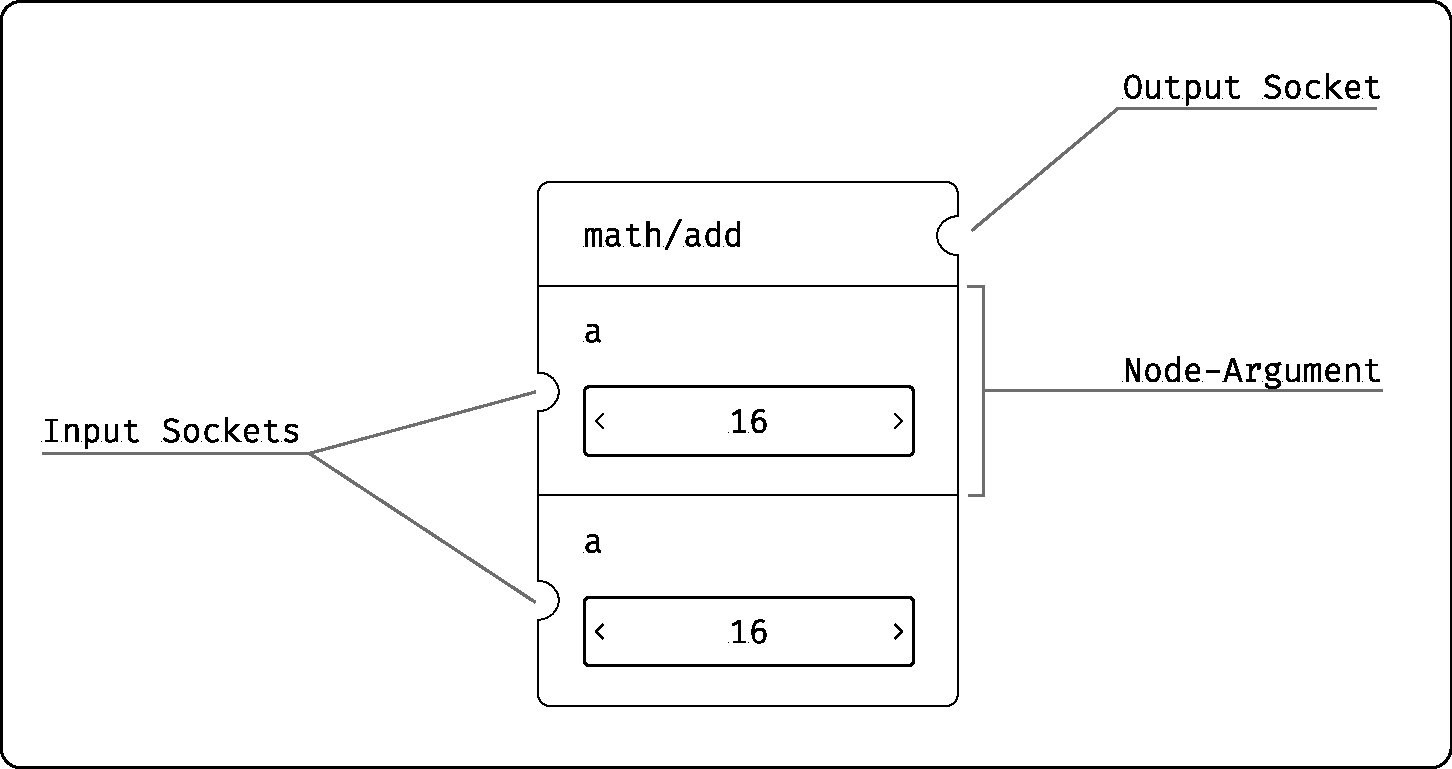
\includegraphics[width=0.47\textwidth]{graphics/NODE_ANATOMY.pdf}
    \caption{Anatomie einer Node}
    \label{sec:NODE_ANATOMY}
\end{wrapfigure}

Das Design der einzelnen Nodes ist stark an das Blender-Design angelehnt. Die Struktur einer Node ist in Abbildung \ref{sec:NODE_ANATOMY} dargestellt. 

Ein deutlich limitierender Faktor beim Design der Nodes ist der vertikale Raum, den eine Node einnimmt. Da bei der Entwicklung einer Node die Anzahl der Argumente schnell anwachsen kann, kann auch die vertikale Größe schnell anwachsen. 
Um dieses Problem zu beheben, wurde den \link[node_input]{Node-Inputs} eine Einstellung hinzugefügt, die diesen Input in ein Untermenü auf der rechten Seite versteckt. 
\end{minipage}
\br
\endgroup

\begin{figure}[htpb]
  \centering
  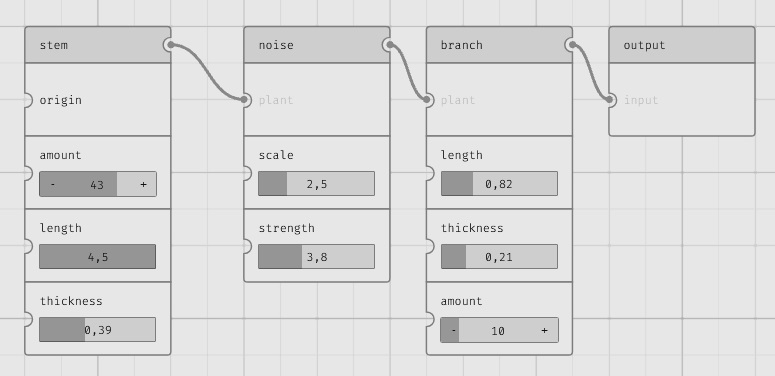
\includegraphics[width=1\textwidth]{graphics/node_graph.jpg}
  \caption{Screenshot eines \link[node_graph]{Node-Graphen}}
  \label{fig:node_graph_screenshot}
\end{figure}

\pagebreak

\section{Implementierung}
Die Anwendung wurde in einem Mono-Repository entwickelt, das die einzelnen Komponenten als eigenständige Pakete enthält. Dies hat den Vorteil, dass alle Komponenten gemeinsam entwickelt, versioniert und getestet werden können. \cite{GithubRepo}
\br
Außerdem unterstützen die beiden Paket-Manager \href{https://pnpm.io/}{pnpm} und \href{https://crates.io/}{cargo} das Arbeiten mit 
Mono-Repositories sehr gut. 
\br
Des Weiteren wurde nach dem Prinzip des Interface-Driven-Development vorgegangen, das heißt die Interfaces der einzelnen Komponenten wurde vor ihrer Implementierung festgelegt. Das hilft, die Interfaces so minimal wie möglich zu halten und so auch die Kopplung zwischen den Komponenten zu minimieren.

\subsection{Nodes}
Die Nodes wurden als Cargo-Pakete entwickelt. Jede Node ist ein eigenes Rust-Projekt und wird als WebAssembly-Modul kompiliert.
\br
Jede Node hat zwei öffentliche Funktionen, \topic{execute} und \topic{get\_definition}. Die \topic{execute} Funktion nimmt einen Array aus 32-Bit-Integer entgegen und gibt ein Array aus 32-Bit-Integer zurück. 
\br
Die \topic{get\_definition} Funktion gibt die \link[node_definition]{Node-Definition} der Node zurück. 
Diese \link[node_definition]{Node-Definition} wird in einer JSON-Datei definiert, die dann über ein prozedurales Rust-Macro geladen, validiert und in die WebAssembly-Datei eingebettet wird. Dies stellt sicher, dass eine Node nur erfolgreich kompiliert werden kann, wenn die \link[node_definition]{Node-Definition} valide ist.

\subsection{Runtime-Executor}
Der Runtime-Executor wurde als TypeScript Klasse mit einer \topic{execute} Funktion implementiert. Diese \topic{execute} Funktion nimmt ein \link[node_graph]{Node-Graph} entgegen und gibt ein Array aus 32-Bit-Integer zurück. Die Funktion ist grob in folgende Schritte eingeteilt:

\begin{enumerate}
  \item Finde eine Node mit dem Typ \topic{output}
  \item Finde rekursiv alle Nodes, die mit dieser Node verbunden sind
  \item Sortiere diese Nodes nach ihrer Entfernung zur \topic{output}-Node, von der am weitesten entfernten zur am nächsten entfernten
  \item Führe die Nodes in dieser Reihenfolge aus
\end{enumerate}

Das Ausführen der einzelnen Nodes läuft etwa wie folgt ab:

\begin{enumerate}
  \item Für jeden Input der Node:
  \begin{enumerate}
      \item Wenn der Input mit einer anderen Node verbunden ist, nutze das Ergebnis dieser Node
      \item Wenn nicht, nutze den Wert, der über das \link[node_interface]{Node-Interface} festgelegt wurde
  \end{enumerate}
  \item Enkodiere die Argumente der Node mit der \link[code_nested_encoding]{Binär-Serialisierung}
  \item Führe die \topic{execute}-Funktion der Node mit den Argumenten aus
\end{enumerate}

\subsection{Node-Interface}
Der Fokus bei der Implementierung lag darauf, das Interface so simpel und performant wie möglich zu gestalten. Hierfür wurde eine hybride Darstellung aus HTML- und WebGL-Elementen entwickelt. HTML-Elemente bieten den Vorteil, dass sie einfach zu gestalten sind und über gute Interaktionsmöglichkeiten verfügen. Bei einer großen Anzahl sich bewegender HTML Elemente sinkt jedoch die Performance. 
Deshalb wird ab einer bestimmten Zoom-Stufe die Darstellung der Nodes in ein WebGL Canvas gerendert. Dies hat den Vorteil, dass die Performance bei einer großen Anzahl von Nodes konstant bleibt. 
\br
Zur weiteren Verbesserung der Performance werden die abgerundeten Ecken und Rahmen der einzelnen Nodes per \href{https://en.wikipedia.org/wiki/Signed_distance_function}{Signed-Distance-Function} gerendert. So werden für jede Node nur vier Vertices und zwei Polygone benötigt. Auch die Verbindungen zwischen den Nodes werden als WebGL-Elemente gerendert.

Um das Arbeiten mit dem Interface so effizient wie möglich zu gestalten, wurden einige Funktionen implementiert:

\subsubsection{Drag-and-Drop}
WebAssembly-Dateien können per Drag-and-Drop in das Interface geladen werden. Die Datei wird validiert, dann in die Node-Registry geladen und die Nodes können im Interface benutzt werden. Außerdem können so auch ganze Node-Graphen geladen werden.

\subsubsection{Selektion}
Das Interface kann jeweils eine aktive Node und mehrere selektierte Nodes haben.
\br
Ähnlich wie in Blender können die Nutzenden eine Box um mehrere Nodes ziehen, um diese auszuwählen. Dafür muss die \topic{strg}-Taste gedrückt gehalten werden und mit gedrückter linker Maustaste eine Box um die gewünschten Nodes gezogen werden.
\br
Mit dem Tastenkürzel \topic{strg + a} können alle Nodes ausgewählt werden. 
\br
Mit der \topic{l}-Taste  werden alle Nodes selektiert die mit der aktiven Node verbunden sind.
\br
Wird \topic{shift} gedrückt wird, während eine Node ausgewählt wird, werden alle Nodes zwischen der aktiven Node und der gewählten Node selektiert.

\subsubsection{Ripple-Delete}
Diese Funktion erlaubt das Löschen einzelner Nodes während die Verbindungen zwischen deren Eltern und Kindern erhalten werden. Das Tastenkürzel ist \topic{strg + x}.

\subsubsection{Hilfsmodus}
Mit dem Tastenkürzel \topic{?} kann der Hilfsmodus aktiviert werden. Hierbei werden dem/der Nutzer/in bei Hover über eine Node die wichtigsten Informationen angezeigt. Dies soll die Einarbeitung in die Anwendung erleichtern.

\subsubsection{Node-Settings}
Da die einzelnen Nodes möglichst wenig Raum einnehmen sollen, können einzelne Inputs von Nodes in ein Untermenü verschoben werden. Dieses zeigt dann jeweils die Inputs der aktiven Node an. 

\subsubsection{Copy/Paste}
Das \link[node_interface]{Node-Interface} unterstützt das Kopieren und Einfügen von Nodes. Dafür werden die Tastenkombinationen \topic{strg + c} und \topic{strg + v} benutzt.

\subsubsection{Undo/Redo}
Die Anwendung verfügt über ein robustes Undo/Redo System. Dank der losen Kopplung der einzelnen Komponenten konnte das System einfach implementiert werden. Es basiert auf der leistungsstarken \hyperref[https://github.com/benjamine/jsondiffpatch]{jsondiffpatch} Bibliothek. Dies hat den Vorteil,  das für jede Aktion nur die Differenz gespeichert wird und nicht der gesamte \link[node_graph]{Node-Graph}.

\pagebreak


\section{Evaluation}

\subsection{Anforderungen}

\subsubsection{Performance}

Die Performance wurde anhand von drei Benchmarks auf drei Geräten jeweils in Chrome (v124) und Firefox (v125) getestet. Die drei Benchmarks im Überblick:

\begin{itemize}
  \item test\_a: 6 Nodes generieren 2,1 Millionen Polygone
  \item test\_b: 228 Nodes generieren 127 Tsd. Polygone
  \item test\_c: 228 Nodes generieren 1 Million Polygone
\end{itemize}

Die drei Geräte waren ein Smartphone (Google Pixel 4a 2020, 8 GB RAM, Snapdragon 730G), ein Laptop (Razer Blade Stealth 2016, 16 GB RAM, i7-7500U) und eine Workstation (Intel I7-6700K, 16 GB RAM, Nvidia GTX1060). 
\br
Die einzelnen Benchmarks wurden end-to-end gemessen. Es wurde also die Zeit gemessen die benötigt wird, um den \link[node_graph]{Node-Graphen} auszuführen, die Polygone in der Szene zu aktualisieren und die Szene zu rendern.
Dargestellt wird die Durchschnittsdauer von 500 Durchläufen sowie die Standardabweichung.

\begin{table}[htbp]
\begin{tabular}{|l|l|l|l|}
\hline
Firefox      & Smartphone                 & Laptop                 & Workstation                 \\ \hline
test\_a      & 208.34ms \stdev{31.51}     & 111ms \stdev{20.76}    & 105.75ms \stdev{12.33}      \\ \hline
test\_b      & 42.07ms \stdev{11.24}      & 22.66ms \stdev{5.63}   & 20.12ms \stdev{3.79}        \\ \hline
test\_c      & 168.66ms \stdev{54.74}     & 67.58ms \stdev{40.03}  & 65.33ms \stdev{13.63}       \\ \hline
\end{tabular}
\end{table}


\begin{table}[htbp]
\begin{tabular}{|l|l|l|l|}
\hline
Chrome           & Smartphone                & Laptop                & Workstation                \\ \hline
test\_a          & 347.02ms  \stdev{30.6}    & 127.97ms \stdev{7.28} & 136.92ms \stdev{3.28}      \\ \hline
test\_b          & 77.19ms \stdev{31.75}     & 21.1ms  \stdev{6.01}  & 18.12ms \stdev{3.74}       \\ \hline
test\_c          & 316.73ms \stdev{62.54}    & 65.46ms \stdev{15.65} & 67.62ms \stdev{23.03}      \\ \hline
\end{tabular}
\end{table}

Die Ergebnisse zeigen, dass auch bei einer großen Anzahl von Nodes und einer hohen Anzahl an Polygonen die Dauer einer Aktualisierung unter 500 ms bleibt. 

\pagebreak

\subsubsection{Erweiterbarkeit}

Wie schnell kann eine neue Node entwickelt, kompiliert und geladen werden? Um dies zu testen wurde eine neue Node entwickelt, die einen Zylinder generiert. 
\br
Erst werden die nötigen Voraussetzungen Rust und wasm-pack installiert.

\begin{figure}[htbp]
  \begin{code}
    \begin{minted}{bash}
$ curl --proto '=https' --tlsv1.2 -sSf https://sh.rustup.rs | sh
$ cargo install wasm-pack
    \end{minted}
  \end{code}
\end{figure}

Dann wird ein bereits bestehendes Template für eine Node kopiert und die Implementierung angepasst. 

\begin{figure}[htbp]
  \begin{code}
    \begin{minted}{bash}
$ git clone --depth=1 https://github.com/jim-fx/nodarium_template new-node
$ cd new-node
    \end{minted}
  \end{code}
\end{figure}


Nun legt man die Node-Definition an, dafür wird die Datei \topic{src/definition.json} angepasst. Hier ist die Definition für die Zylinder-Node:


\begin{figure}[htbp]
  \begin{code}
    \begin{minted}{json}
{
  "id": "my-name/my-namespace/zylinder-node",
  "outputs": [
    "geometry"
  ],
  "inputs": {
    "height": {
      "type": "float",
      "value": 2,
    },
    "radius": {
      "type": "float",
      "value": 0.4
    }
  }
}
    \end{minted}
  \end{code}
\end{figure}

Danach wird die Implementierung in der Datei \topic{src/lib.rs} angepasst. Der \link[code_cylinder_node]{Beispiel-Code} zeigt deutlich, dass wenig Boilerplate-Code benötigt wird. Ein Großteil der Implementierung lag darin, den Code zu schreiben, der die Zylinder-Geometrie generiert.  Außerdem kann das gesamte Rust-Ökosystem genutzt werden, so zum Beispiel \href{https://docs.rs/glam/latest/glam}{glam}, eine Bibliothek für Vektoren und Matrizen.

\pagebreak

Nun wird die Node mit dem folgenden Befehl kompiliert:

\begin{figure}[htbp]
  \begin{code}
    \begin{minted}{bash}
$ wasm-pack build --release
    \end{minted}
  \end{code}
\end{figure}

Die kompilierte Node liegt unter \topic{pkg/new\_nodarium\_node.wasm}. Bei diesem Beispiel ist sie etwa 28 KB groß. Zum Laden der Node wird diese per Drag-and-Drop in die Anwendung geladen. 
\br
Alles in allem hat die Entwicklung und das Laden der Node etwa 30 Minuten gedauert. Die meiste Zeit wurde für die Implementierung der Zylinder-Geometrie benötigt. 
Durch die Validierung der Node-Definition durch das prozedurale \topic{include\_definition\_file} Rust-Macro und die vielen Hilfsfunktionen die in der \topic{nodarium} Bibliothek enthalten sind, ist es sehr einfach eine neue Node zu implementieren.

\subsubsection{Usability}

Durch das einheitliche Design und die Implementierung vielen Hilfsfunktionen ist das \link[node_interface]{Node-Interface} sehr einfach und intuitiv zu bedienen. Zu diesen Funktionen zählen etwa eine Tastaturkürzel-Übersicht, ein Hilfsmodus, ein High-Contrast-Modus und viele weitere.
\br
Um die Usability umgehend zu testen, wären Nutzer-Tests sinnvoll. Diese wurden jedoch nicht durchgeführt, da es bei der Entwicklung der Anwendung in erster Linie um technische Funktionalität ging und der zeitliche Rahmen für Nutzer-Tests nicht ausreichte.

\subsection{Forschungsfragen}

Die beiden Forschungsfragen waren:

\begin{itemize}
  \item Inwieweit eignet sich WebAssembly als Grundlage für eine node-basierte visuelle Programmiersprache?  
  \item Welche Auswirkungen haben die spezifischen Vor- und Nachteile von WebAssembly auf die Realisierbarkeit, Funktionalität, Nutzerfreundlichkeit, Performance, Flexibilität und Robustheit einer solchen Programmiersprache?
\end{itemize}

\subsubsection{WebAssembly als Grundlage}
Die Implementierung der Anwendung hat gezeigt, dass die Vorteile, die WebAssembly bietet die \link[parameter_nodes]{Komplexität der Implementierung}, die durch die Nachteile entstehen, weit überwiegen. Durch Bibliotheken und Frameworks wie \href{https://rustwasm.github.io/wasm-bindgen/}{wasm-bindgen} und \href{https://rustwasm.github.io/wasm-pack/book/}{wasm-pack} ist die Implementierung einer WebAssembly-Anwendung relativ einfach. 
\br
Des Weiteren existiert diese Komplexität nur in der Implementierung und die Endnutzer/innen der Anwendung profitieren ausschließlich von den Vorteilen.

\subsubsection{Vor- und Nachteile von WebAssembly}
\textbf{Realisierbarkeit} beschreibt wie einfach es ist, die Anwendung zu implementieren. Hier entsteht durch die Low-Level-Natur von WebAssembly eine gewisse Komplexität. 
Da WebAssembly allerdings keine neue Technologie ist, existieren bereits Tools und Bibliotheken, die viele dieser Probleme lösen.
\br
\textbf{Funktionalität} beschreibt, welchen Einfluss die Nutzung von WebAssembly auf die Umsetzung der Anforderung der Anwendung hat. Hierbei wird deutlich, dass die Nutzung von WebAssembly bei der Optimierung der \textbf{Performance} hilft, da es erlaubt, die unterliegenden Hardware-Ressourcen besser zu nutzen.
\br
\textbf{Flexibilität} beschreibt, wie einfach es ist die Anwendung zu erweitern. Auch hier ist WebAssembly eine gute Wahl, da unterschiedliche Sprachen zu WebAssembly kompilieren können und so Entwickler/innen die Wahl haben, welche Sprache sie nutzen wollen. Besonders die Eigenschaft, dass WebAssembly Module self-contained sind und keine Annahmen über die Umgebung machen, erhöht die Flexibilität.

\section{Fazit}
Anhand der Analysen der vorher definierten Anforderung und der Evaluation der Forschungsfragen lässt sich sagen, dass die Anwendung die Anforderungen erfüllt und die Forschungsfragen beantwortet sind.
\br
WebAssembly eignet sich trotz der Komplexität gut als Grundlage für die Implementierung einer node-basierten visuellen Programmiersprache. Die Vorteile, die WebAssembly bietet, wie die Performance, die Flexibilität und die Robustheit, überwiegen die Nachteile, wie die Komplexität und die schwierigen Debugging-Möglichkeiten. Ein weiterer großer Vorteil ist, dass jede Node eine einzelne WebAssembly-Datei ist, was die Anwendung sehr modular macht und die Erweiterbarkeit erhöht.

\section{Ausblick}
Bei der Entwicklung der Anwendung entstanden eine Reihe von Ideen und Konzepten, die in der aktuellen Version nicht umgesetzt wurden, da 
diese entweder den zeitlichen Rahmen gesprengt hätten oder nicht in den Kontext dieser Arbeit passten.

\subsection*{Hosted-Node-Registry}
Aus Gründen der Einfachheit und der Performance wurde die Node-Registry als Teil der Anwendung implementiert. Da aber eines der Ziele der Anwendung die Erweiterbarkeit ist, wäre es sinnvoll, die Node-Registry als eigenständigen Service zu implementieren. Die Anwendung wurde bereits so implementiert, dass dies ohne Änderung an bestehenden Komponenten möglich ist.
\br
Dies ist aber ein recht komplexes Unterfangen, da es nicht nur die Implementierung eines Servers, sondern auch die Implementierung von Autorisierung, Authentifizierung und Versionierung erfordert.

\subsection*{WebAssembly-Component-Model}
Wenn das WebAssembly-Component-Model in Browsern verfügbar wird, könnte man den \link[runtime_executor]{Runtime-Executor} als einzelnen WebAssembly-Component implementieren. Dieser könnte nun \link[node]{Nodes} als WebAssembly-Module laden und ausführen, so könnte sich der Overhead vermeiden lassen, der durch die Kommunikation zwischen Javascript und WebAssembly entsteht.

\subsection*{Implementation der Namespaces}
Zu diesem Zeitpunkt kommen alle Nodes in der Anwendung aus dem Namespace \topic{max/plantarium}. In der Zukunft könnten mehrere Namespaces implementiert werden, die verschiedene Implementierungen für die gleichen Nodes enthalten. Die Validation dafür wurde noch nicht implementiert und erfordert noch kleinere Änderungen.

\subsection*{Plugins}
Eine spannende Möglichkeit ist die Implementierung der Runtime als Plugin für andere Programme, zum Beispiel Blender. Dies würde es ermöglichen, in der Web-App Pflanzen zu definieren und anhand dieser Definitionen in Blender 3D-Pflanzen zu generieren. Dies erfordert neben der Implementierung eines Plugins die Implementierung eines Backends, das die Projekte speichert, damit das Plugin darauf zugreifen kann.

\subsection*{Weitere Nodes}
Im aktuellen Stadium ist die Anwendung zur Generierung von Pflanzen eher eine Demonstration der Möglichkeiten als ein vollwertiges Tool. Es fehlen noch viele Nodes, die für das Generieren eine vollständige Pflanze benötigt werden. So fehlen die Möglichkeiten Blätter zu generieren, Pflanzen zu texturieren, Wind oder das Abbrechen von Pflanzenteilen zu simulieren – und viele weitere Nodes.

\subsection*{Entwicklung einer visuellen Identität}
Die Anwendung wurde entwickelt, um durch andere Nutzer/innen erweitert zu werden. 
Um diese Nutzer/innen zu erreichen, macht es Sinn, eine kohärente visuelle Identität zu entwickeln.

\subsection*{Erweitern der Dokumentation}
Für Entwickler ist gute Dokumentation ein sehr wichtiger Punkt, wenn es darum geht, ob sie eine Anwendung nutzen oder nicht. 

\pagebreak
\section{Glossar}

\subsection{Node}
\label{sec:node}
Einzelner Baustein eines \hyperref[sec:node_graph]{Node-Graphs}. Eine Node funktioniert etwa wie eine Funktion in einer textuellen Programmiersprache. Sie nimmt \hyperref[sec:node_argumente]{Node-Argumente} entgegen, verarbeitet diese und gibt ein Ergebnis zurück. 


\subsection{Node-Definition}
\label{sec:node_definition}
Eine Node ist quasi eine Instanz einer Node-Definition. Eine Node-Definition definiert die Struktur einer Node. Sie enthält Informationen über die Inputs und Outputs einer Node und die Funktion, die die Node ausführt.

\subsection{Node-Graph}
\label{sec:node_graph}
Node-Graphs sind gerichtete \link[PURE_GRAPH]{azyklische Graphen (DAG)} von \link[node]{Nodes}. Sie bestehen aus einer Vielzahl von Nodes und deren Verknüpfungen. 

\subsection{Node-Argumente}
\label{sec:node_argumente}
Node-Argumente sind die Eingabeparameter einer Node. Ein Node-Argument kann entweder direkt über das Interface in einer \link[node]{Node} definiert werden oder indem der User einen Output-Socket einer anderen Node mit dem \link[node_socket]{Node-Socket} eines Node-Argument verknüpft.

\subsection{Node-Socket}
\label{sec:node_socket}
Node-Sockets sind die Verbindungspunkte zwischen \link[node]{Nodes}. Eine Node hat mehrere Input-Sockets und einen Output Socket.

\pagebreak

\section{Beispiel-Code}
\subsection{Binär-Serialisierung}
\label{sec:code_nested_encoding}

\begin{figure}[htbp]
  \begin{code}
    \begin{minted}{typescript}
// Recursiver Datenstruktur für verschachtelte Arrays
type SparseArray = (number | number[] | SparseArray<T>)[];

// Kodiert ein verschachteltes Array
export function encodeNestedArray(array: SparseArray): number[] {
  const encoded = [0, 0]; // Initialisiere das Ergebnis
  let missingBracketIndex = 1; // Abstand zur letzten Klammer

  for (let index = 0; index < array.length; index++) {
    const item = array[index];
    if (Array.isArray(item)) {
      // Aktualisiere die letzte Klammer
      encoded[missingBracketIndex] = encoded.length - missingBracketIndex;
      if (item.length === 0) {
        // Behandle leere Arrays
        encoded.push(0, 1, 1, 1);
      } else {
        // Kodiere rekursiv nicht-leere Arrays
        const child = encodeNestedArray(item);
        encoded.push(...child);
      }
      // Aktualisiere den Abstand für die zuletzt geöffnete Klammer
      missingBracketIndex = encoded.length - 1;
    } else {
      // Behandle Nicht-Array-Elemente
      encoded.push(item);
      // Aktualisiere den Abstand für die zuletzt geöffnete Klammer
      if (missingBracketIndex) encoded[missingBracketIndex] = index + 2;
    }
  }

  return [...encoded, 1, 1];
};
    \end{minted}
  \end{code}

  \caption{Beispiel-Code Binär-Serialisierung (TypeScript)}
  \label{sec:data_nested_encoding}

\end{figure}

\pagebreak

\subsection{Binär-Splitting}
\label{sec:code_nested_splitting}

\begin{figure}[htbp]
  \begin{code}
    \begin{minted}{rust}
pub fn split_args(args: &[i32]) -> Vec<&[i32]> {
    let mut out_args: Vec<&[i32]> = Vec::new();
    let mut depth = 0;
    let mut i = 0;
    let mut start_index = 0;
    let mut next_bracket_index = 0;
    let len = args.len();

    while i < len {
        // Wenn wir uns an einer Klammer befinden
        if i == next_bracket_index {
            next_bracket_index = i + args[i + 1] as usize + 1;
            // Wenn die Klammer öffnet
            if args[i] == 0 {
                if depth == 1 {
                    start_index = i;
                }
                depth += 1;
            } else {
                depth -= 1;
                if depth == 1 {
                    out_args.push(&args[start_index..i + 2]);
                    start_index = i + 2;
                }
            }
            i += 2;
            continue;
        } else if depth == 1 {
            out_args.push(&args[i..i + 1]);
            start_index = i + 1;
        }
        i += 1;
    }

    out_args
}
    \end{minted}
  \end{code}

  \caption{Beispiel-Code Binär-Splitting (Rust)}

\end{figure}

\pagebreak

\subsection{Binär-Joining}
\label{sec:code_nested_joining}
\begin{figure}[htbp]
  \begin{code}
    \begin{minted}{rust}
pub fn concat_args(data: Vec<&[i32]>) -> Vec<i32> {
    // 4 um die erste/letzte Klammer zu berücksichtigen
    let mut total_length = 4; 

    for vec in &data { // Berechnen der Gesamtlänge, um Neuzuweisungen zu vermeiden
        if vec.len() == 1 {
            total_length += 1;
        } else {
            total_length += vec.len(); // +4 für die Klammern um jeden Subarray
        }
    }

    let mut result = Vec::with_capacity(total_length);

    result.push(0); // Öffnende Klammer
    result.push(1);

    let mut last_closing_bracket = 1;

    for vec in data.iter() {
        if vec.len() == 1 {
            result.push(vec[0]);
            result[last_closing_bracket] += 1;
            continue;
        } else {
            result.extend_from_slice(vec);
            last_closing_bracket = result.len() - 1;
            result[last_closing_bracket] = 1;
        }
    }

    result.push(1); // Schließende Klammer
    result.push(1);

    result
}

    \end{minted}
  \end{code}

  \caption{Beispiel-Code Binär-Joining (Rust)}

\end{figure}

\pagebreak

\subsection{Zylinder Node}
\label{sec:code_cylinder_node}
\begin{figure}[htbp]
  \fontsize{9}{11}
  \begin{code}
    \begin{minted}{rust}
use glam::Vec2;
use wasm_bindgen::prelude::*;

nodarium_macros::include_definition_file!("src/definition.json");

#[wasm_bindgen]
pub fn execute(input: &[i32]) -> Vec<i32> {
    let arguments = nodarium_utils::split_args(input);
    let height = nodarium_utils::evaluate_float(arguments[0]);
    let radius = nodarium_utils::evaluate_float(arguments[1]);
    let mut geometry_data = nodarium_utils::geometry::create_geometry_data(16, 16);
    let geometry = nodarium_utils::geometry::wrap_geometry_data(&mut geometry_data);

    for i in 0..8 {
        let x = radius * (2.0 * std::f32::consts::PI * i as f32 / 8.0).cos();
        let y = radius * (2.0 * std::f32::consts::PI * i as f32 / 8.0).sin();
        let vec = Vec2::new(x, y).normalize();

        geometry.positions[i * 3 + 0] = x;                // Untere Punkte des Cylinders
        geometry.positions[i * 3 + 1] = 0.0;
        geometry.positions[i * 3 + 2] = y;
        geometry.normals[i * 3 + 0] = vec[0];
        geometry.normals[i * 3 + 1] = 0.0;
        geometry.normals[i * 3 + 2] = vec[1];
        geometry.positions[24 + i * 3 + 0] = x;           // Obere Punkte des Cylinders
        geometry.positions[24 + i * 3 + 1] = height;
        geometry.positions[24 + i * 3 + 2] = y;
        geometry.normals[24 + i * 3 + 0] = vec[0];
        geometry.normals[24 + i * 3 + 1] = 0.0;
        geometry.normals[24 + i * 3 + 2] = vec[1];
        geometry.faces[i * 6 + 0] = (i + 8) as i32;       // Festlegen der Polygone
        geometry.faces[i * 6 + 1] = (i as i32 + 1) % 8;
        geometry.faces[i * 6 + 2] = (i) as i32;
        geometry.faces[i * 6 + 3] = 8 + (i % 8) as i32;
        geometry.faces[i * 6 + 4] = 8 + (i as i32 + 1) % 8;
        geometry.faces[i * 6 + 5] = (i as i32 + 1) % 8;
    }

    nodarium_utils::concat_arg_vecs(vec![geometry_data]) // Enkodieren des Ergebnisses
}
    \end{minted}
  \end{code}

  \caption{Beispiel-Code Zylinder Node (Rust)}

\end{figure}

\pagebreak
\section{Literaturverzeichnis}

\printbibliography

\end{document}
